\documentclass{article}
\usepackage[utf8]{inputenc}
\usepackage{graphicx}

\title{Laporan Tugas Database 2}
\author{Dian Markuci (1184095)}
\date{1 November 2019}

\begin{document}

\maketitle

\section {\textbf Langkah-langkah Membuat Aplikasi di Oracle Express}\\

\item 1. Masukkan semua data login
\begin{center}
    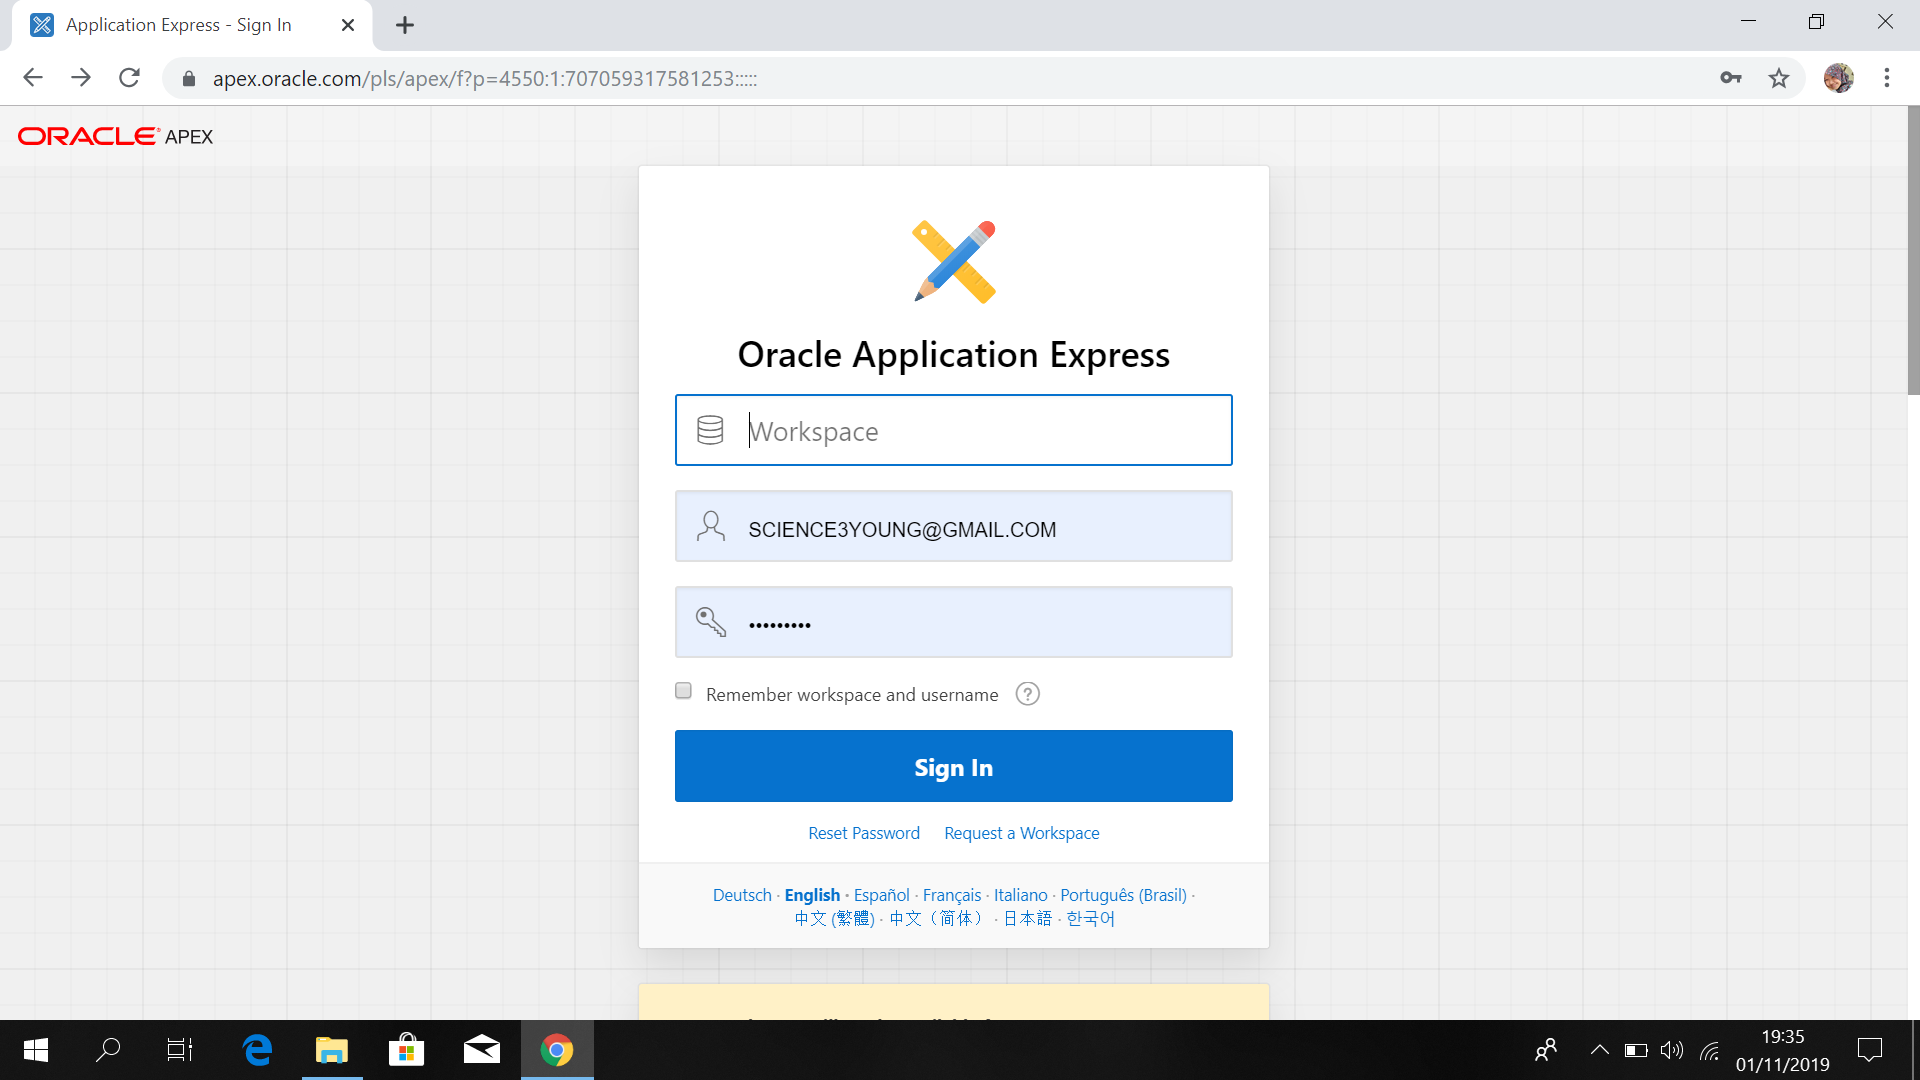
\includegraphics[width=15cm\textwidth]{figure/1login.png}
\end{center}\\

\item 2. Pilih App Builder
\begin{center}
    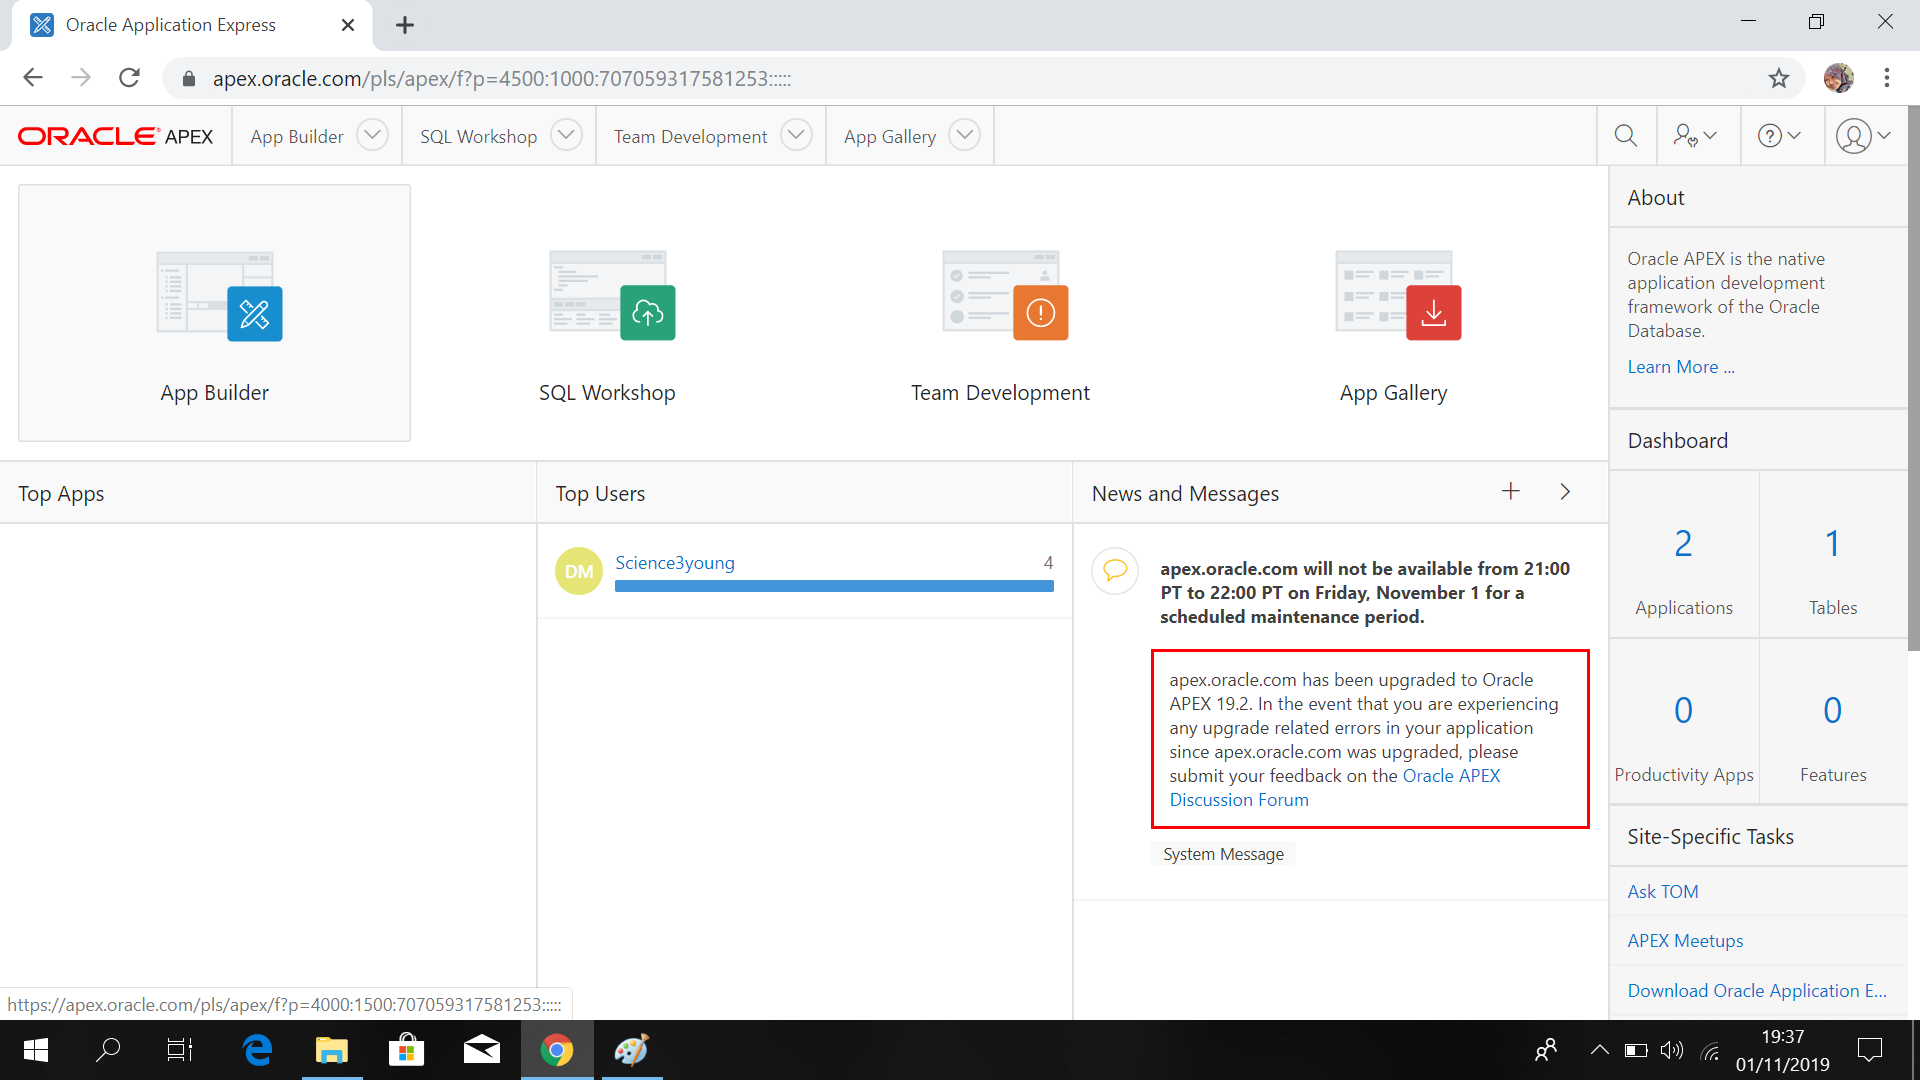
\includegraphics[width=15cm\textwidth]{figure/2Appbuilder.png}\\
\end{center}

\item 3. pilih data dari pc/laptop, lalu pilih create
\begin{center}
    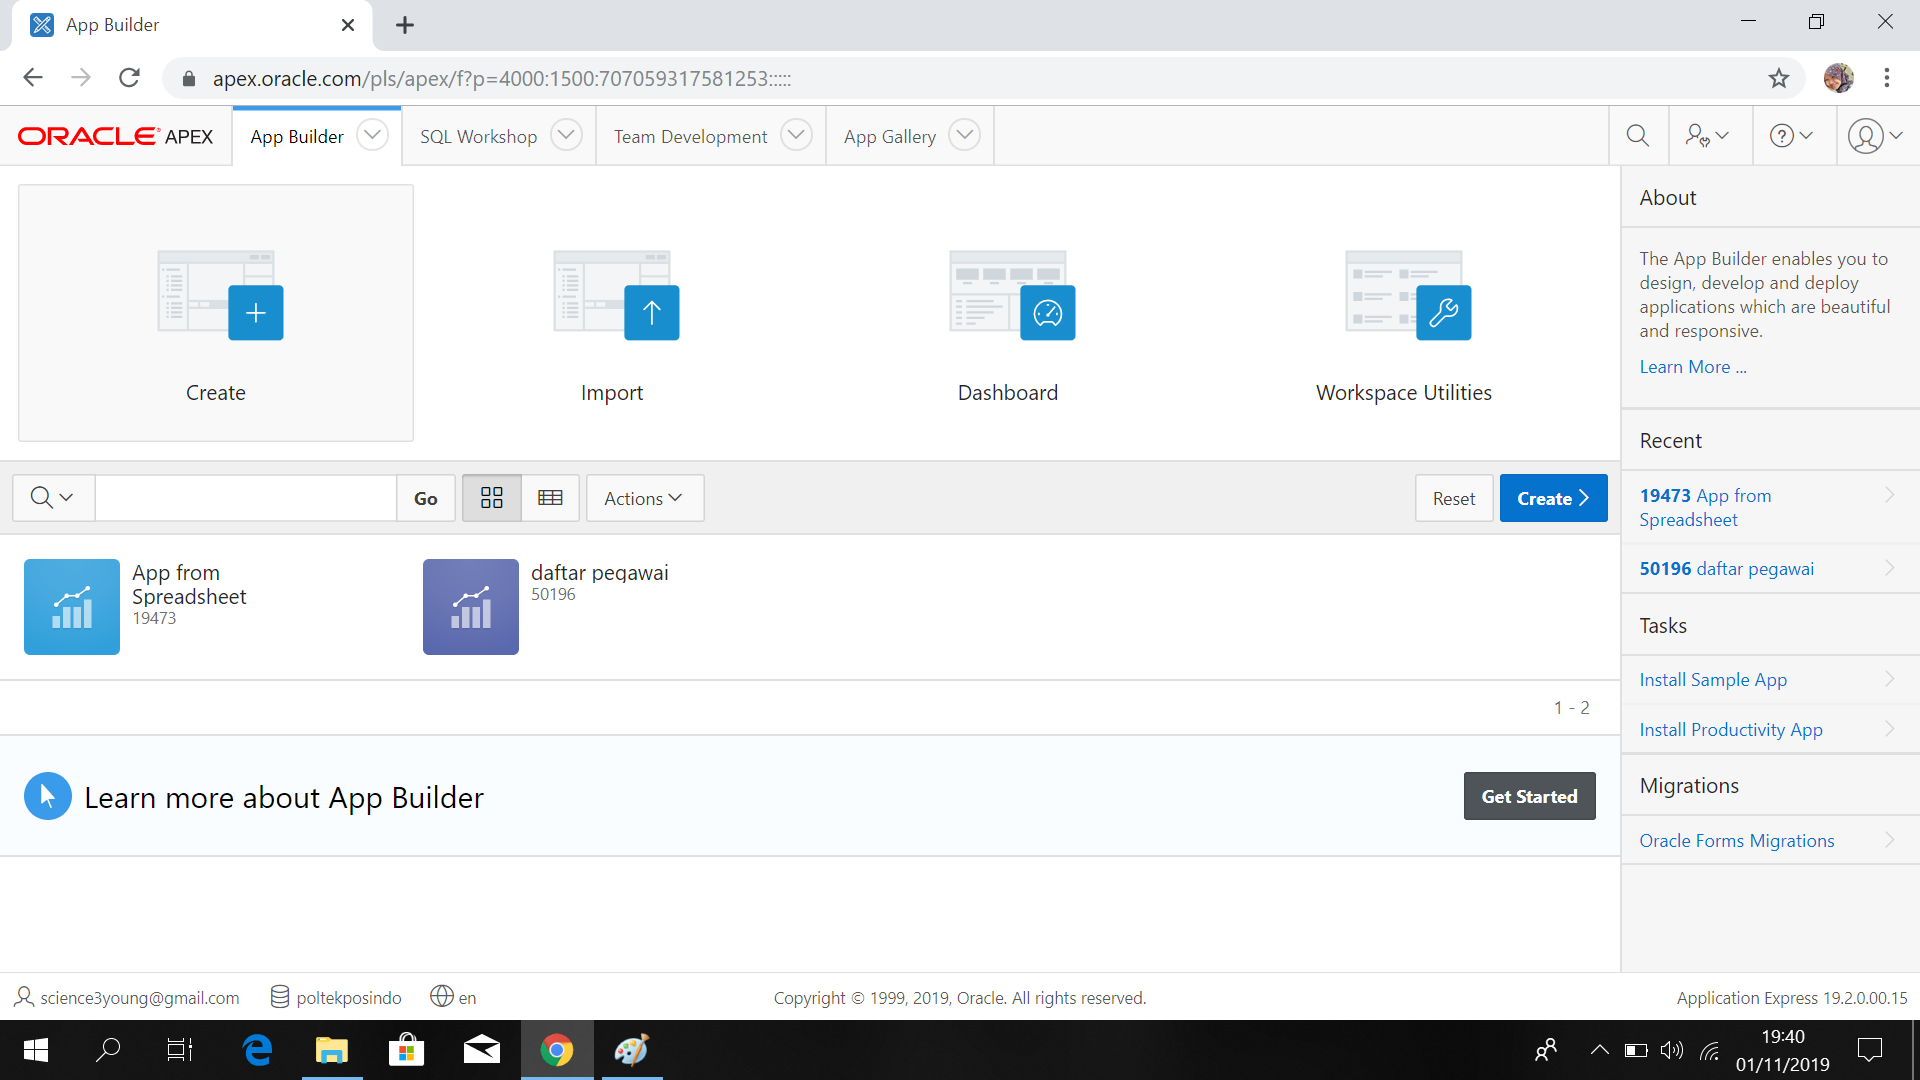
\includegraphics[width=15cm\textwidth]{figure/3Create.png}\\
\end{center}

\item 4. Pilih from a file 
\begin{center}
    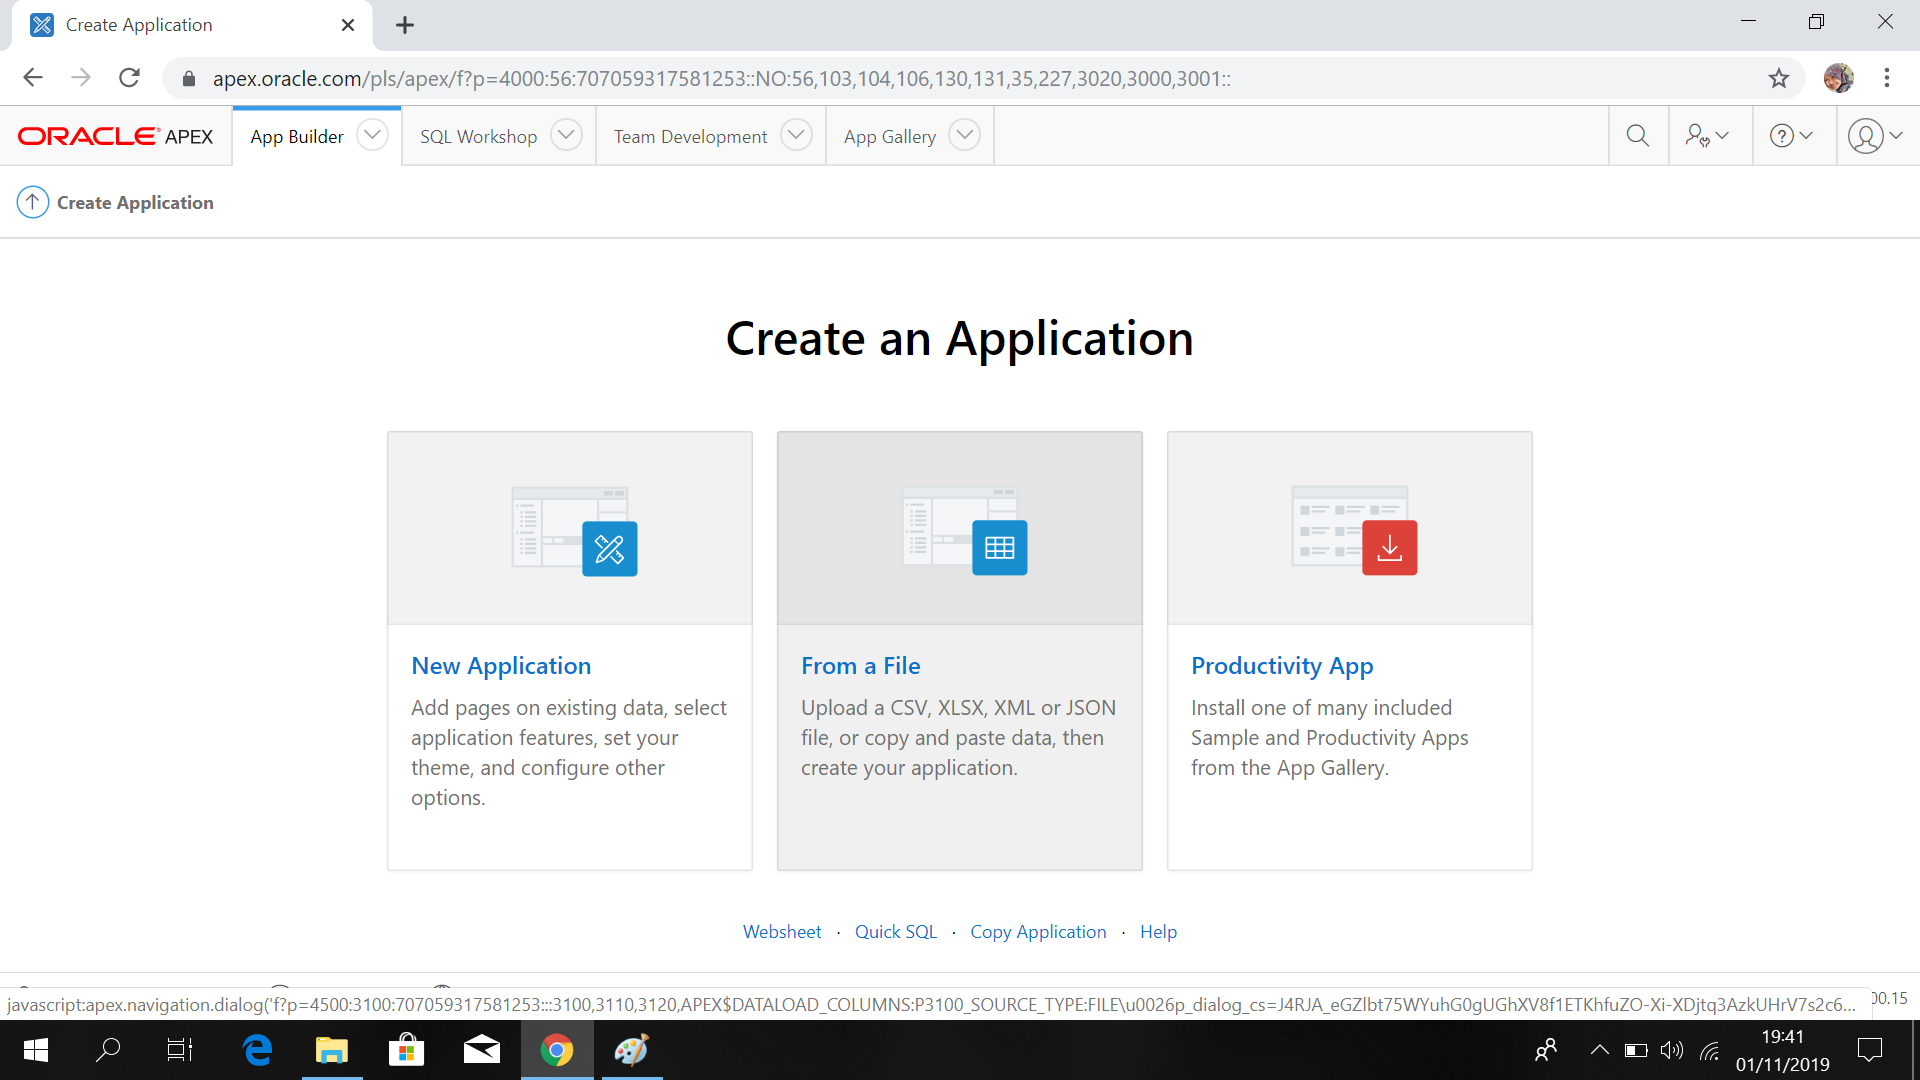
\includegraphics[width=15cm\textwidth]{figure/4from.png}\\
\end{center}

\item 5. klik choose file, masukan file excelnya, create 
\begin{center}
    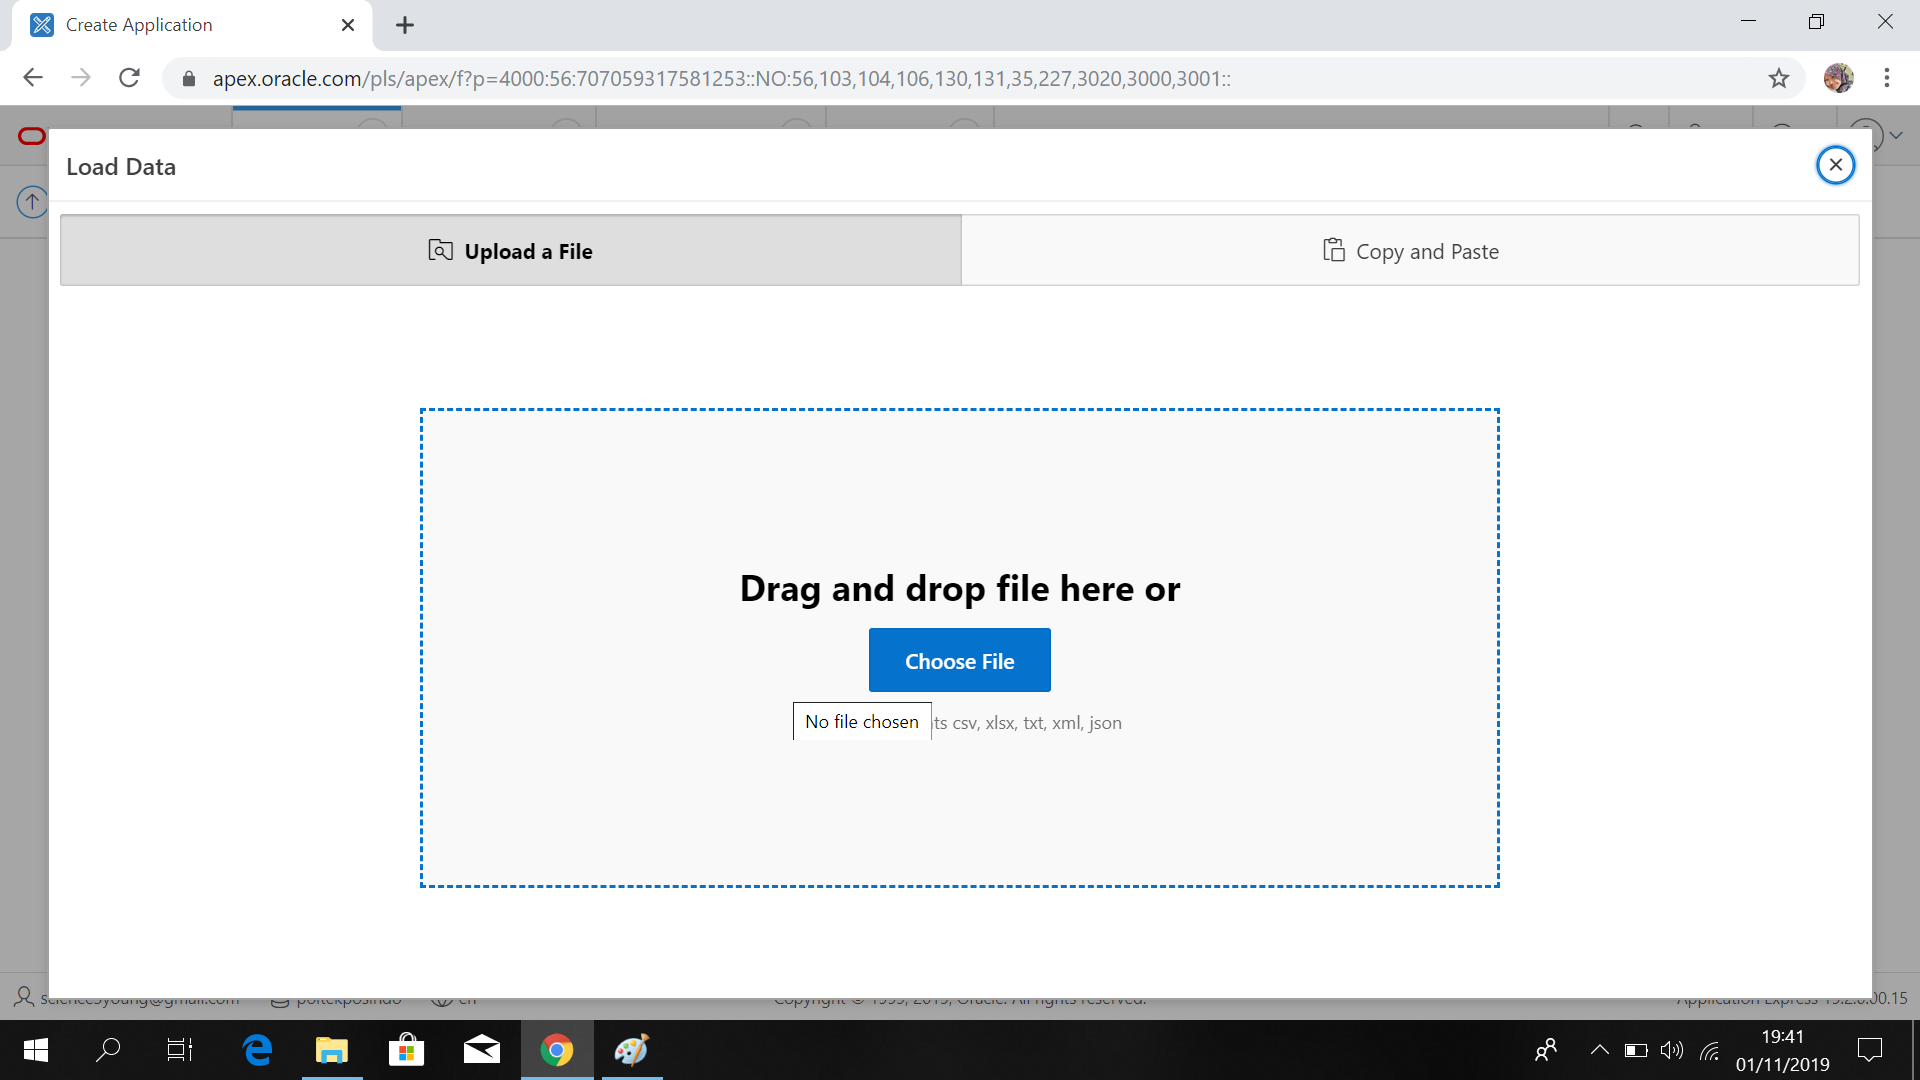
\includegraphics[width=15cm\textwidth]{figure/5choose.png}
\end{center}

\item 6. Setelah kita pilih selanjutnya kita masukkan nama tabelnya lalu klik field error table name hasilnya seperti gambar 
\begin{center}
    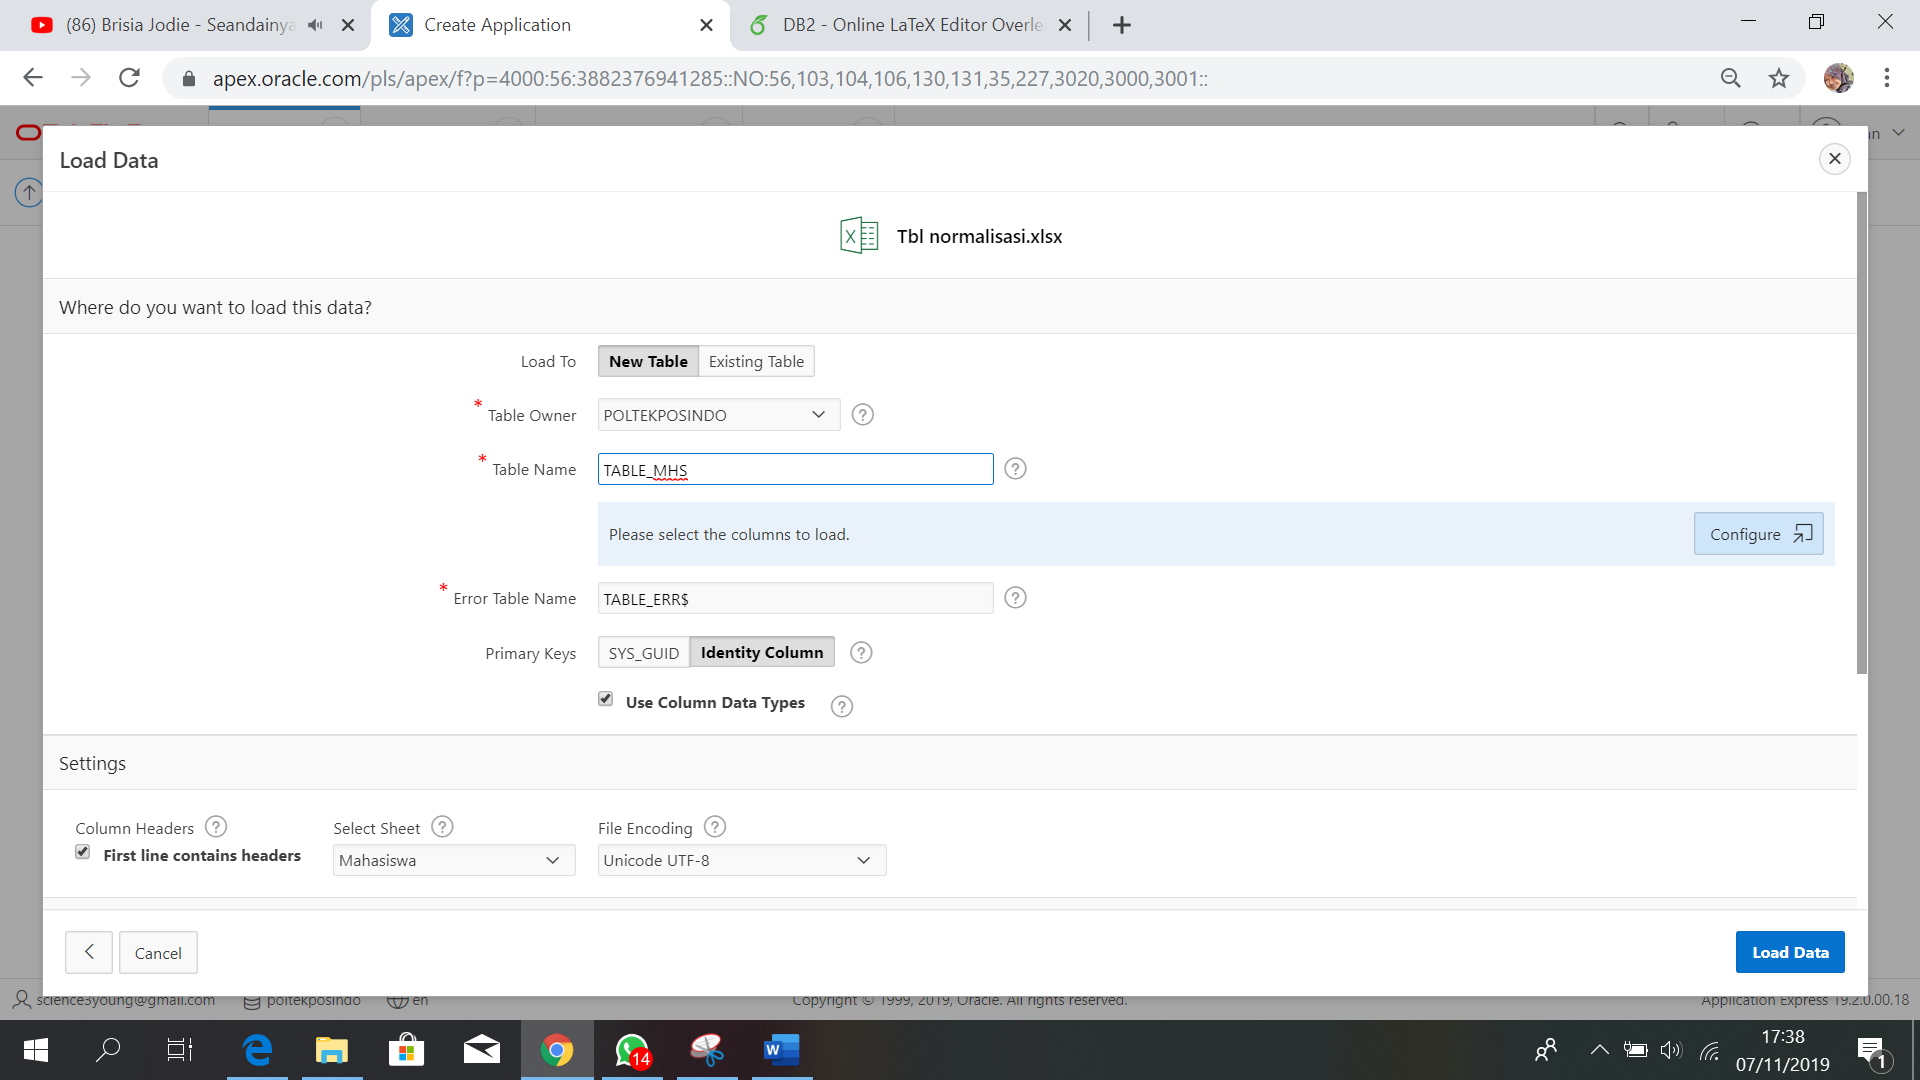
\includegraphics[width=15cm]{figure/isidata1.png}
\end{center}

\item 7. Klik configure untuk memastikan bahwa atribut sudah betul seperti gambar\\
\begin{center}
    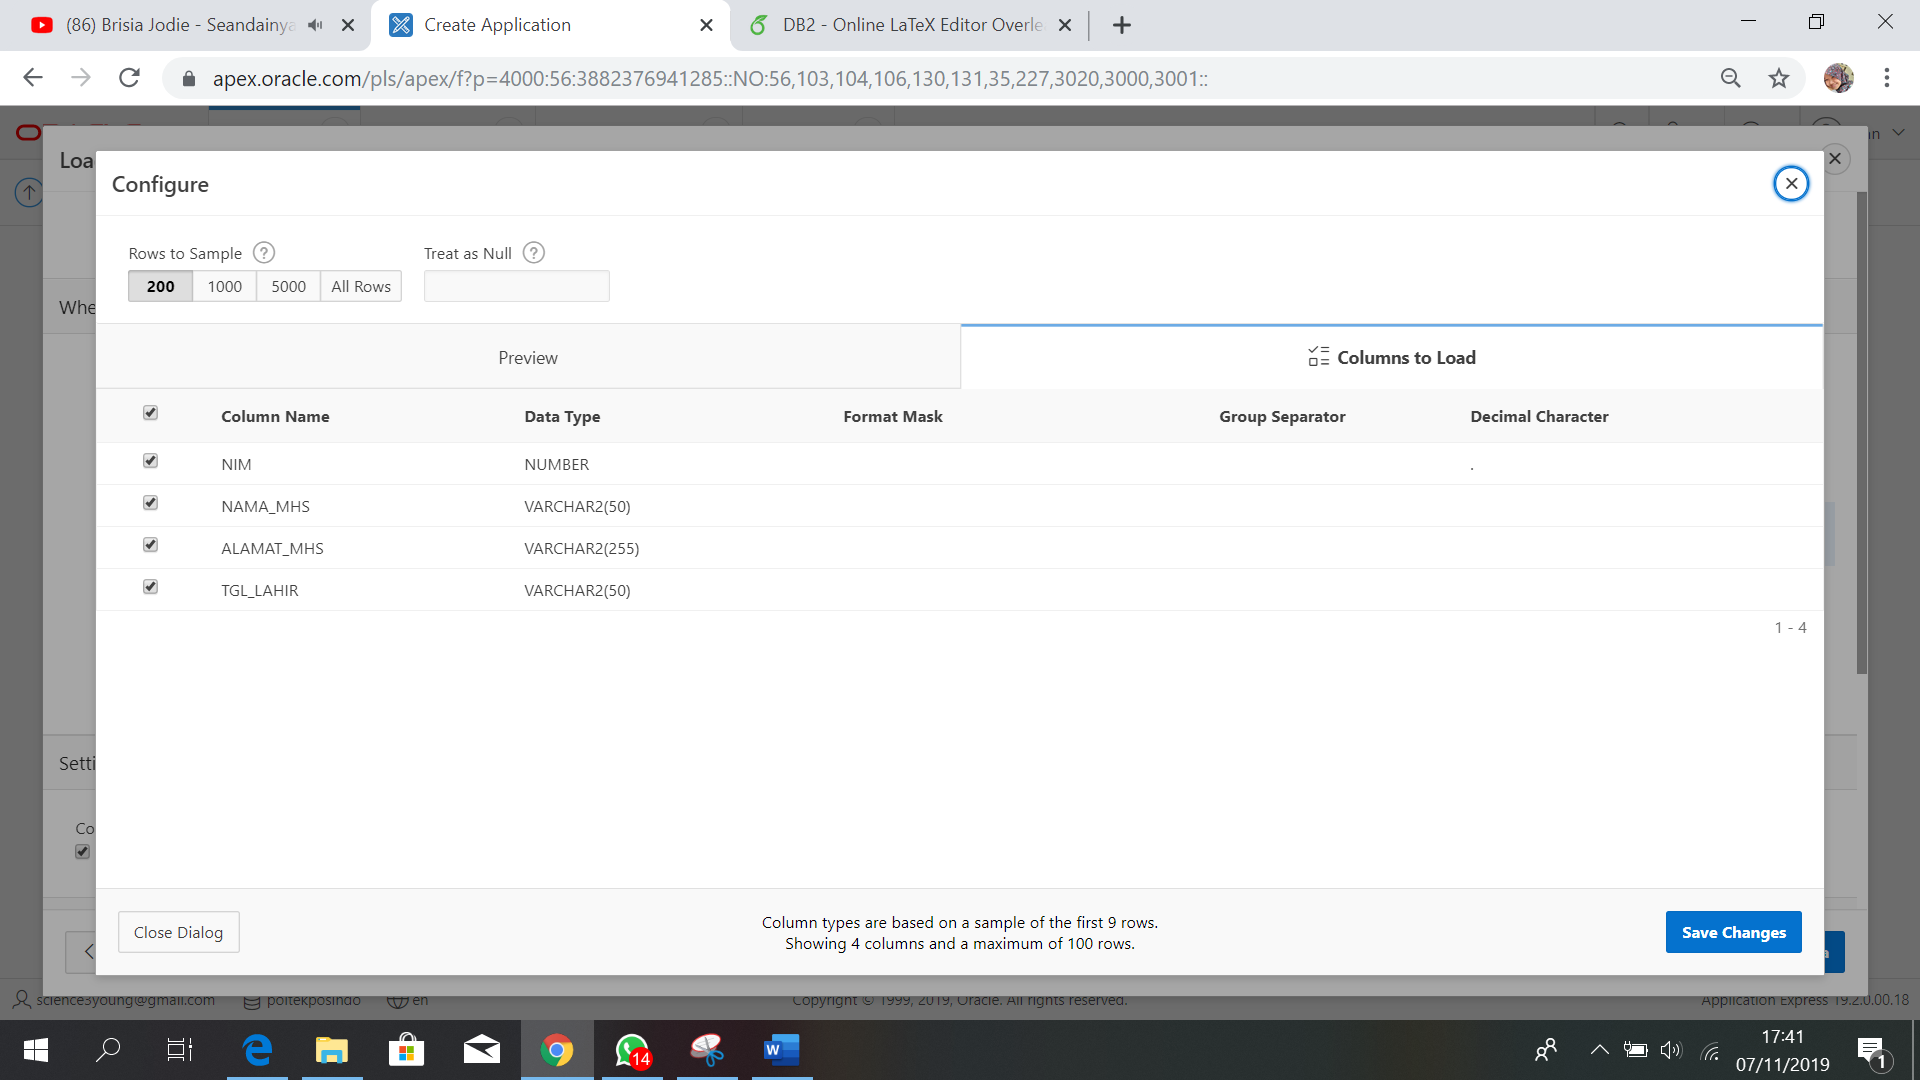
\includegraphics[width=15cm\textwidth]{figure/configure2.png}
\end{center}

\item 8. Klik load dan hasilnya akan seperti :\\
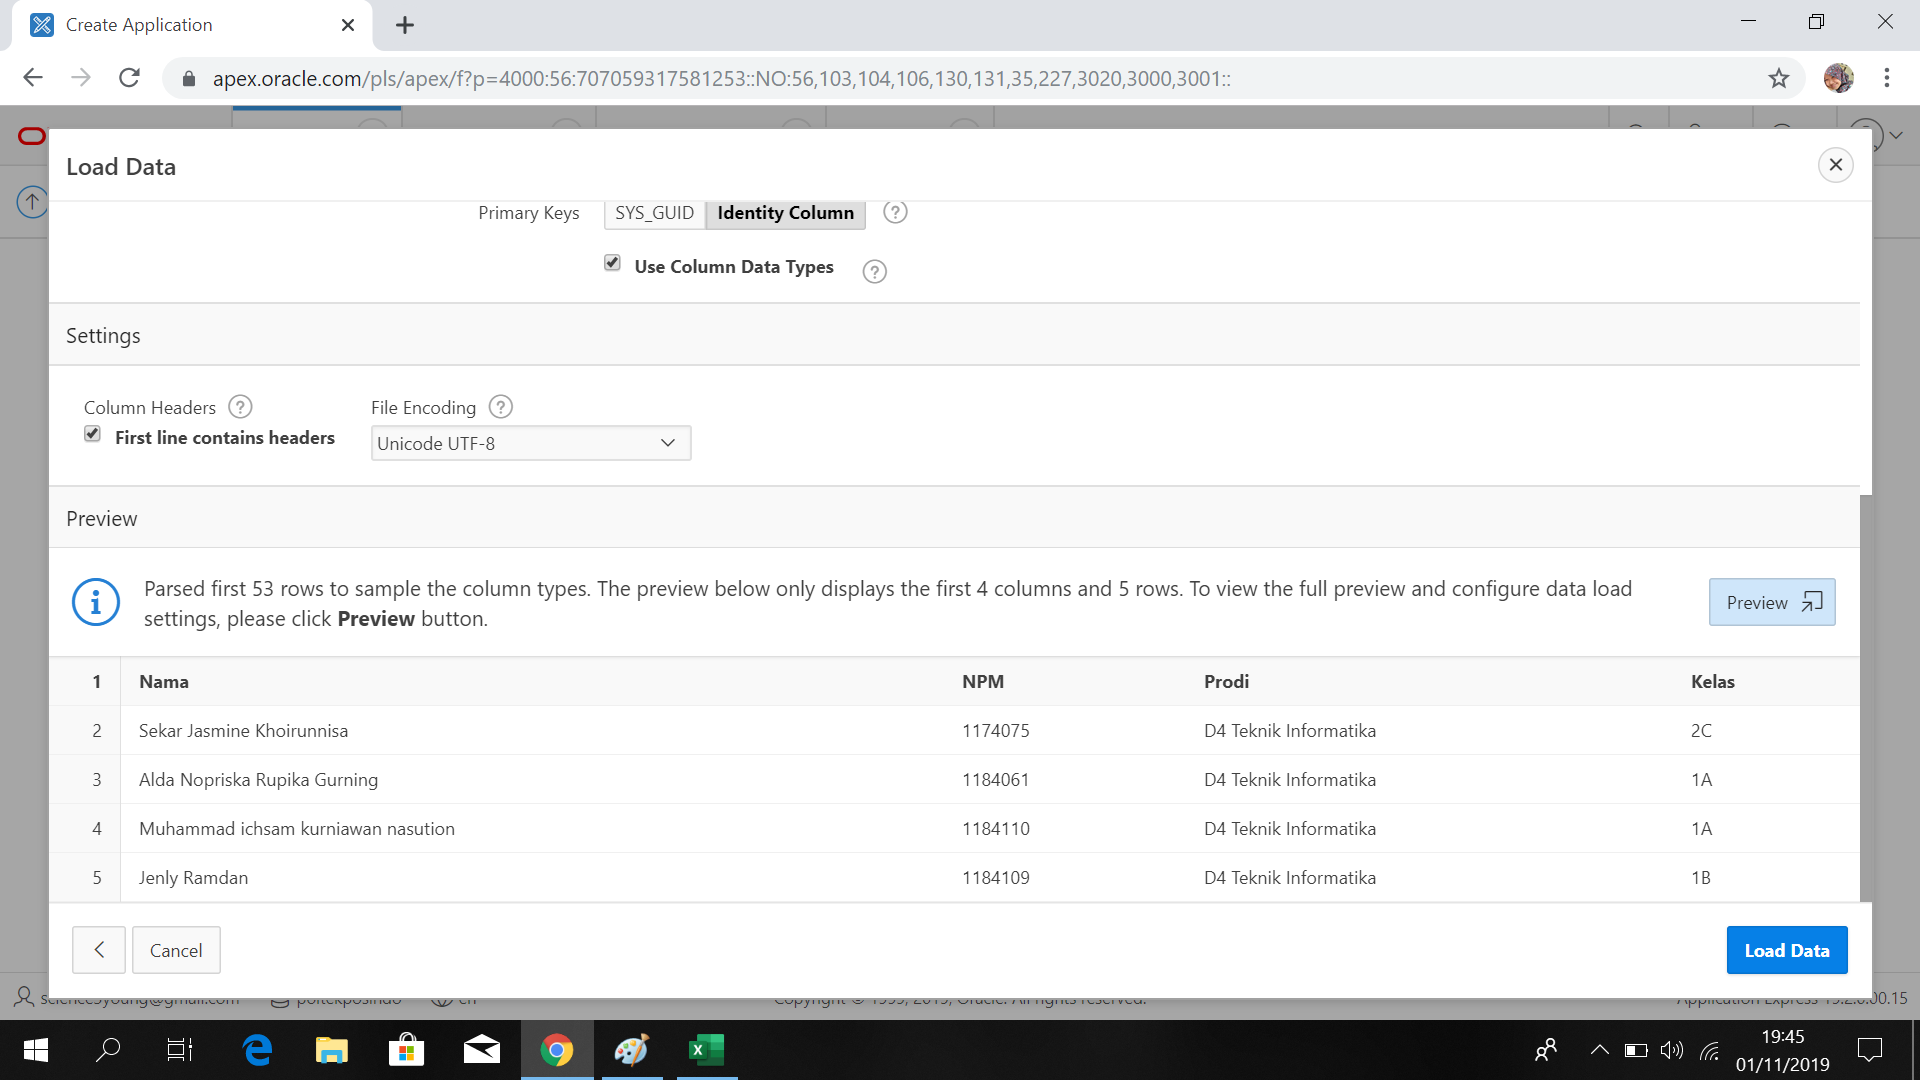
\includegraphics[width=15cm\textwidth]{figure/6load.png}
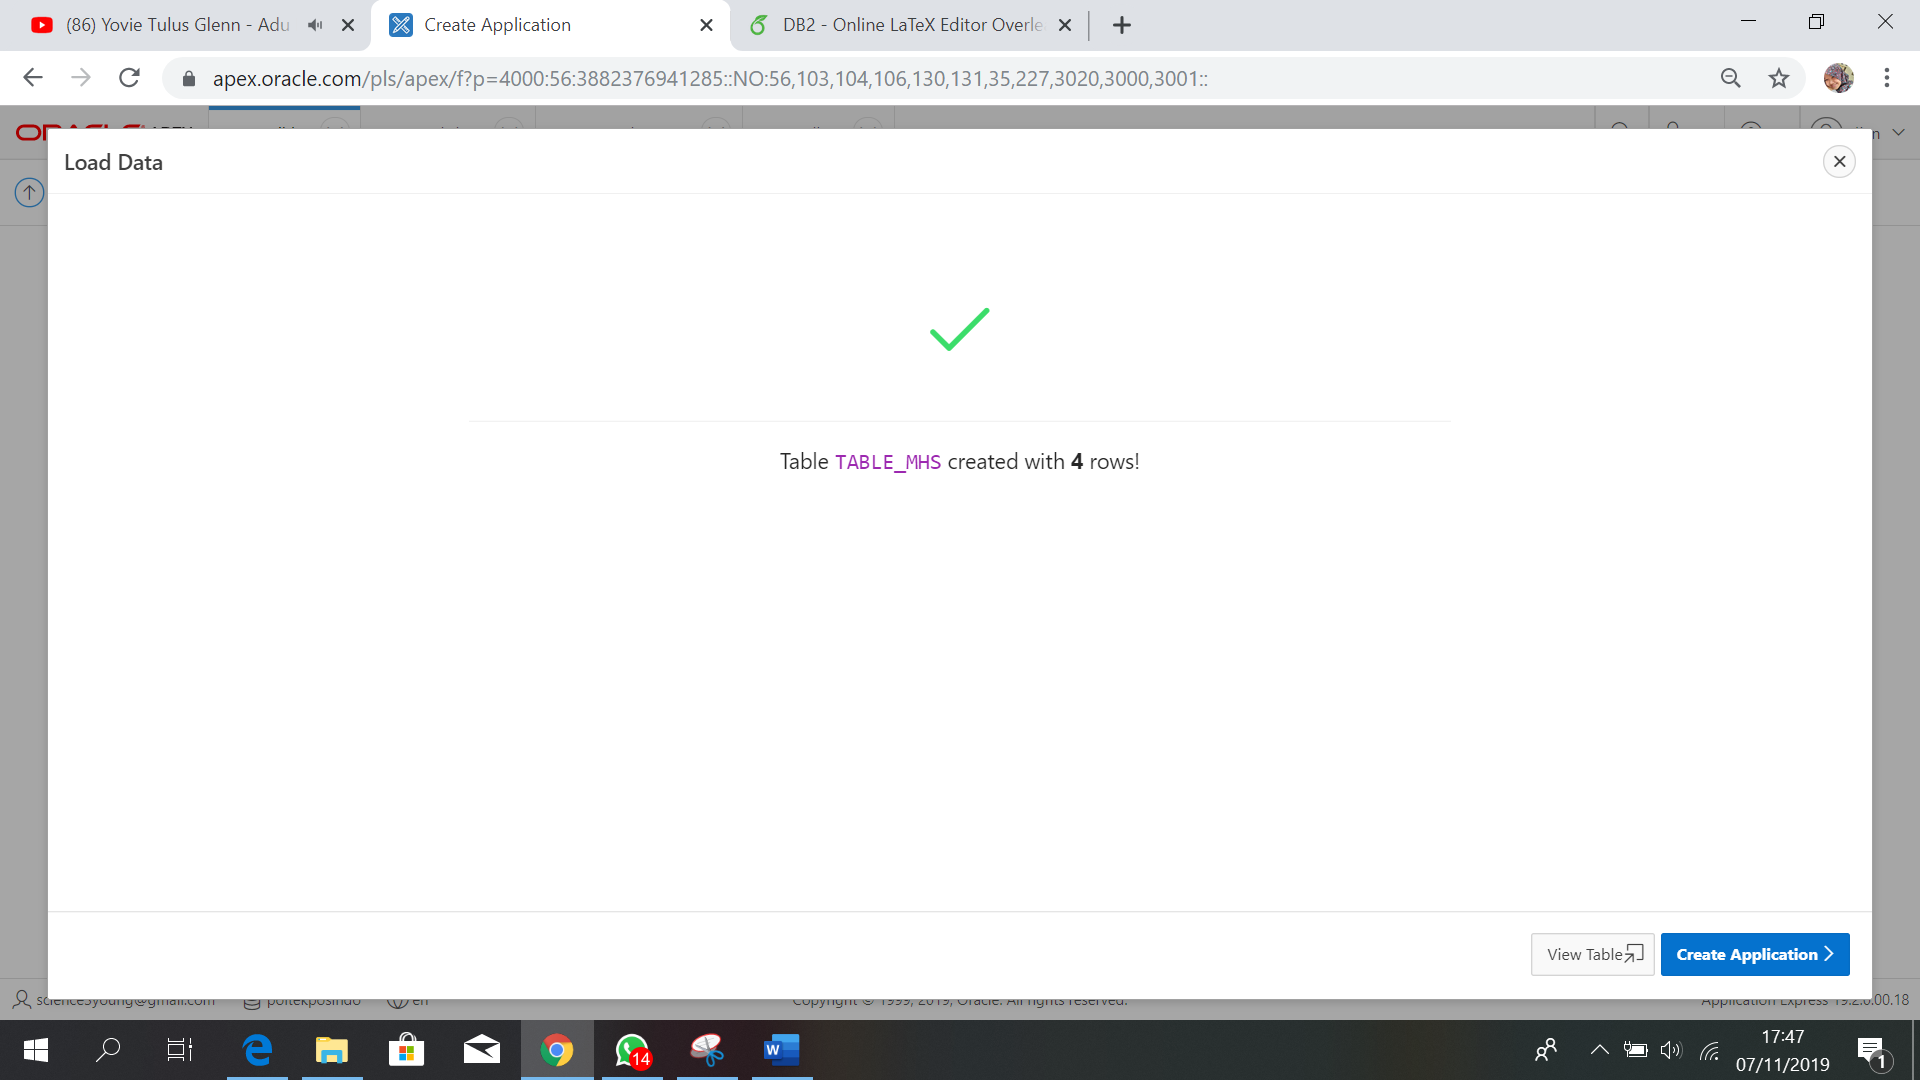
\includegraphics[width=15cm\textwidth]{figure/hasil.png}

\item 9. Lakukan berulang dari tahap 2 hingga tahap 8 sesuai tabel yang diupload\\

\item 10. hapus semua primary key ID menggunakan drop column, dikarenakan ID yang diberikan otomatis oleh sistem apex jika di file kita tidak memiliki primary key\\
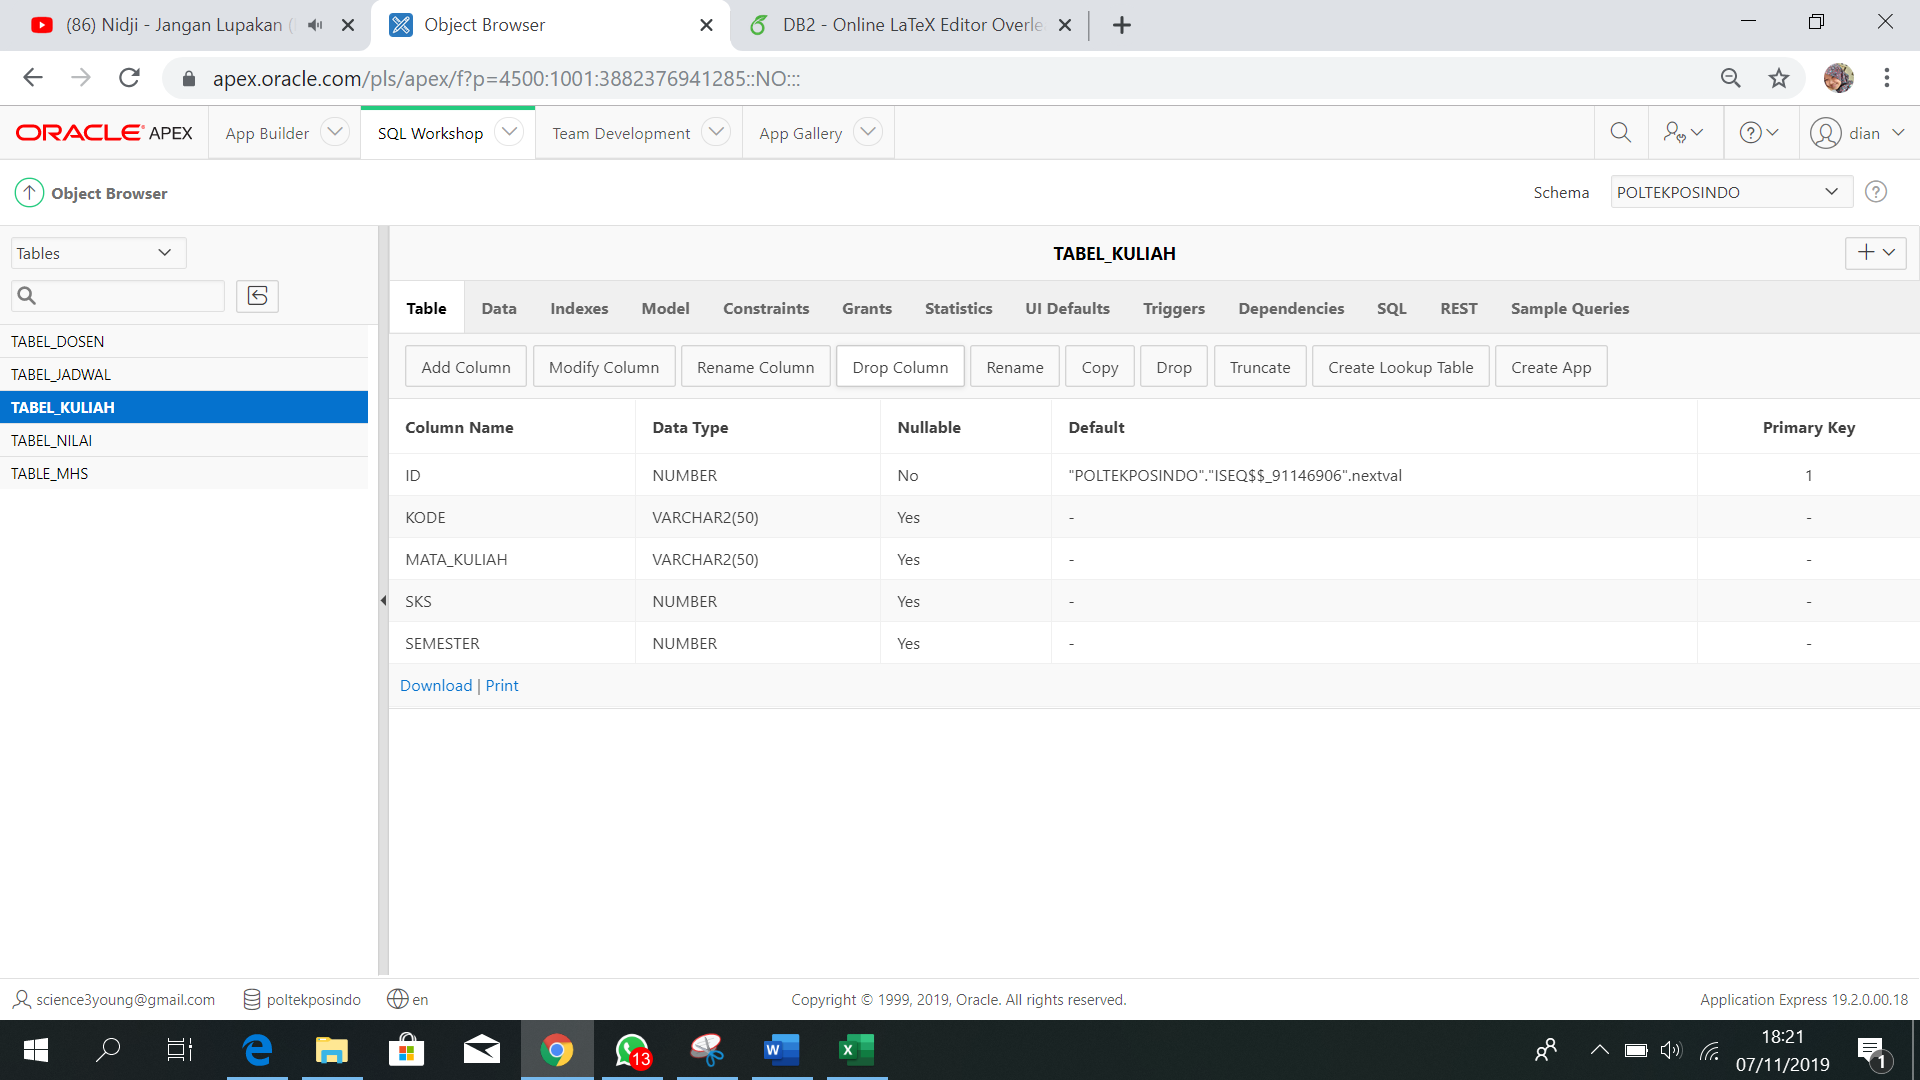
\includegraphics[width=15cm\textwidth]{figure/dropclom.png}

\item 11. Selanjutnya klik sql workshop lalu ke object browser\\
    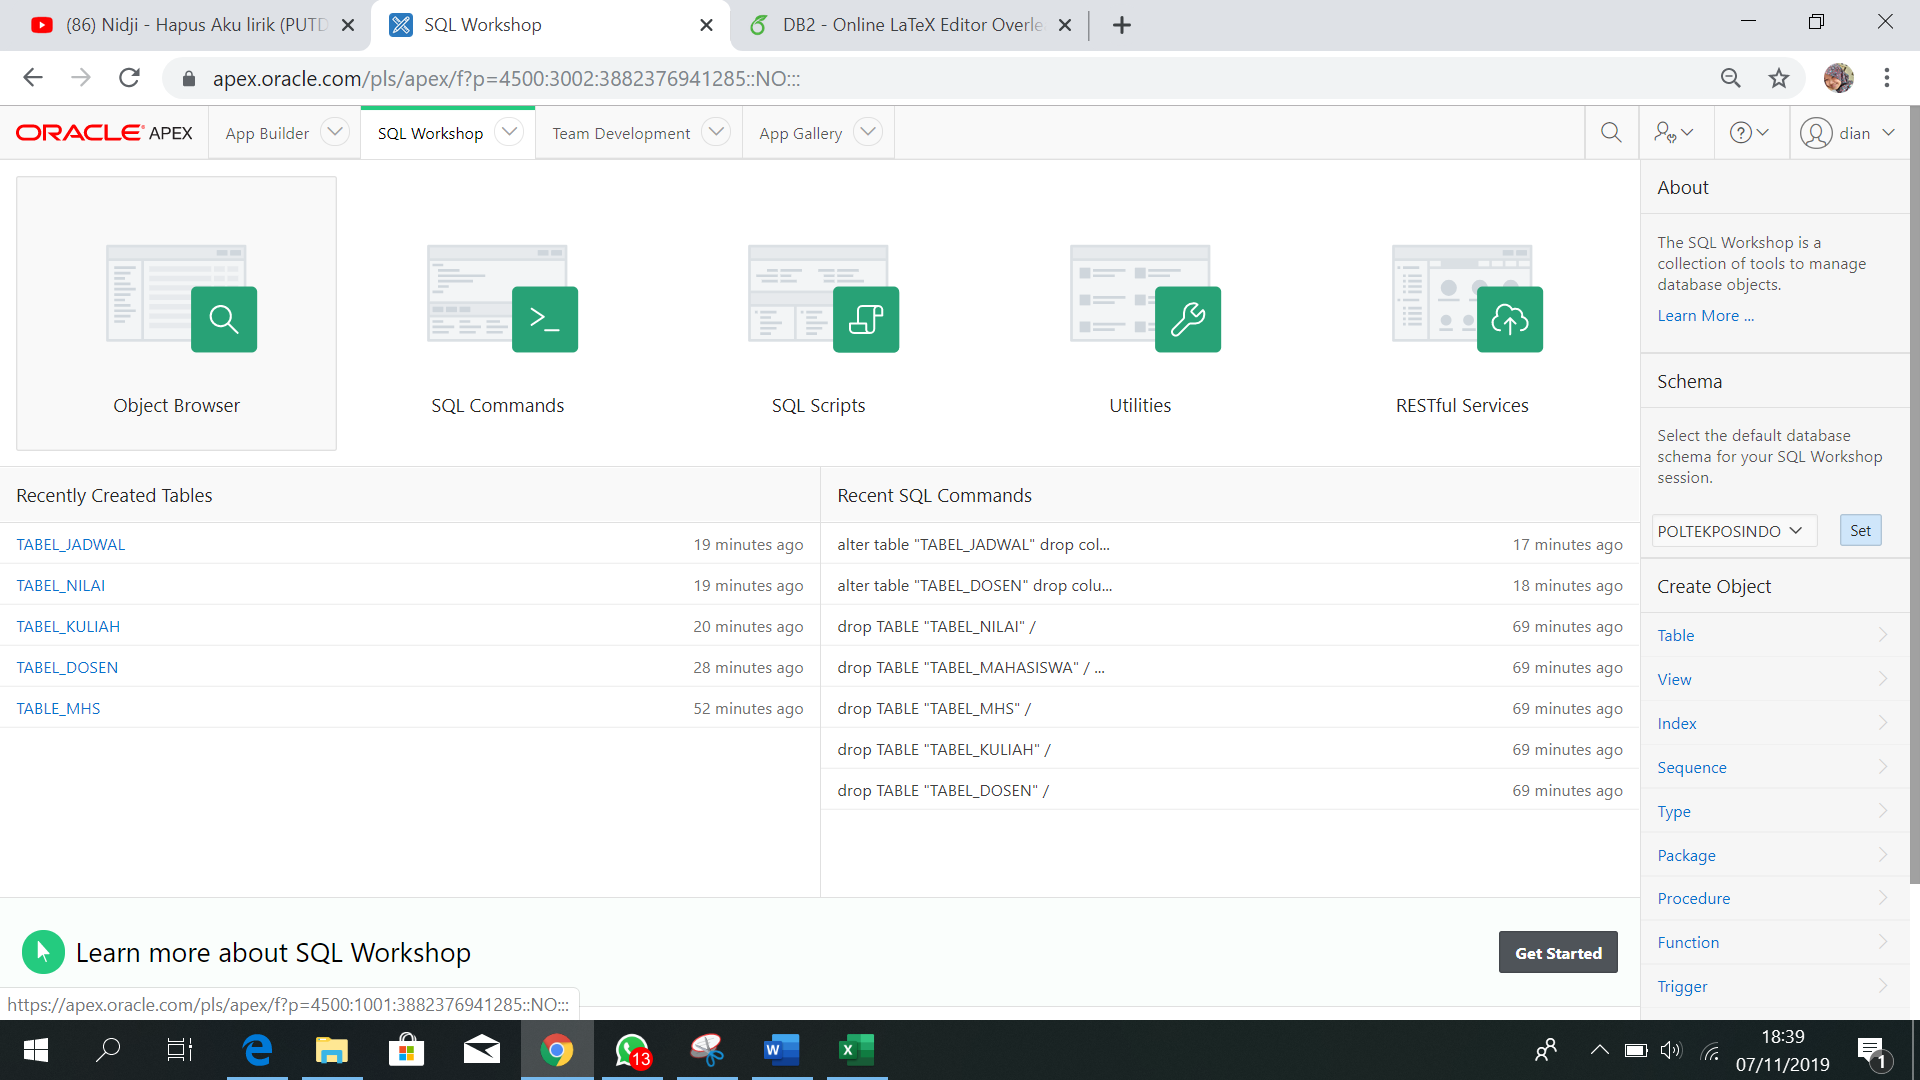
\includegraphics[width=15cm\textwidth]{figure/objectbrow.png}

\item 12.  Setelah itu kita add primary key kesetiap tabel yang telah kita upload. Run dan tunggu hingga muncul pesan table altered.\\

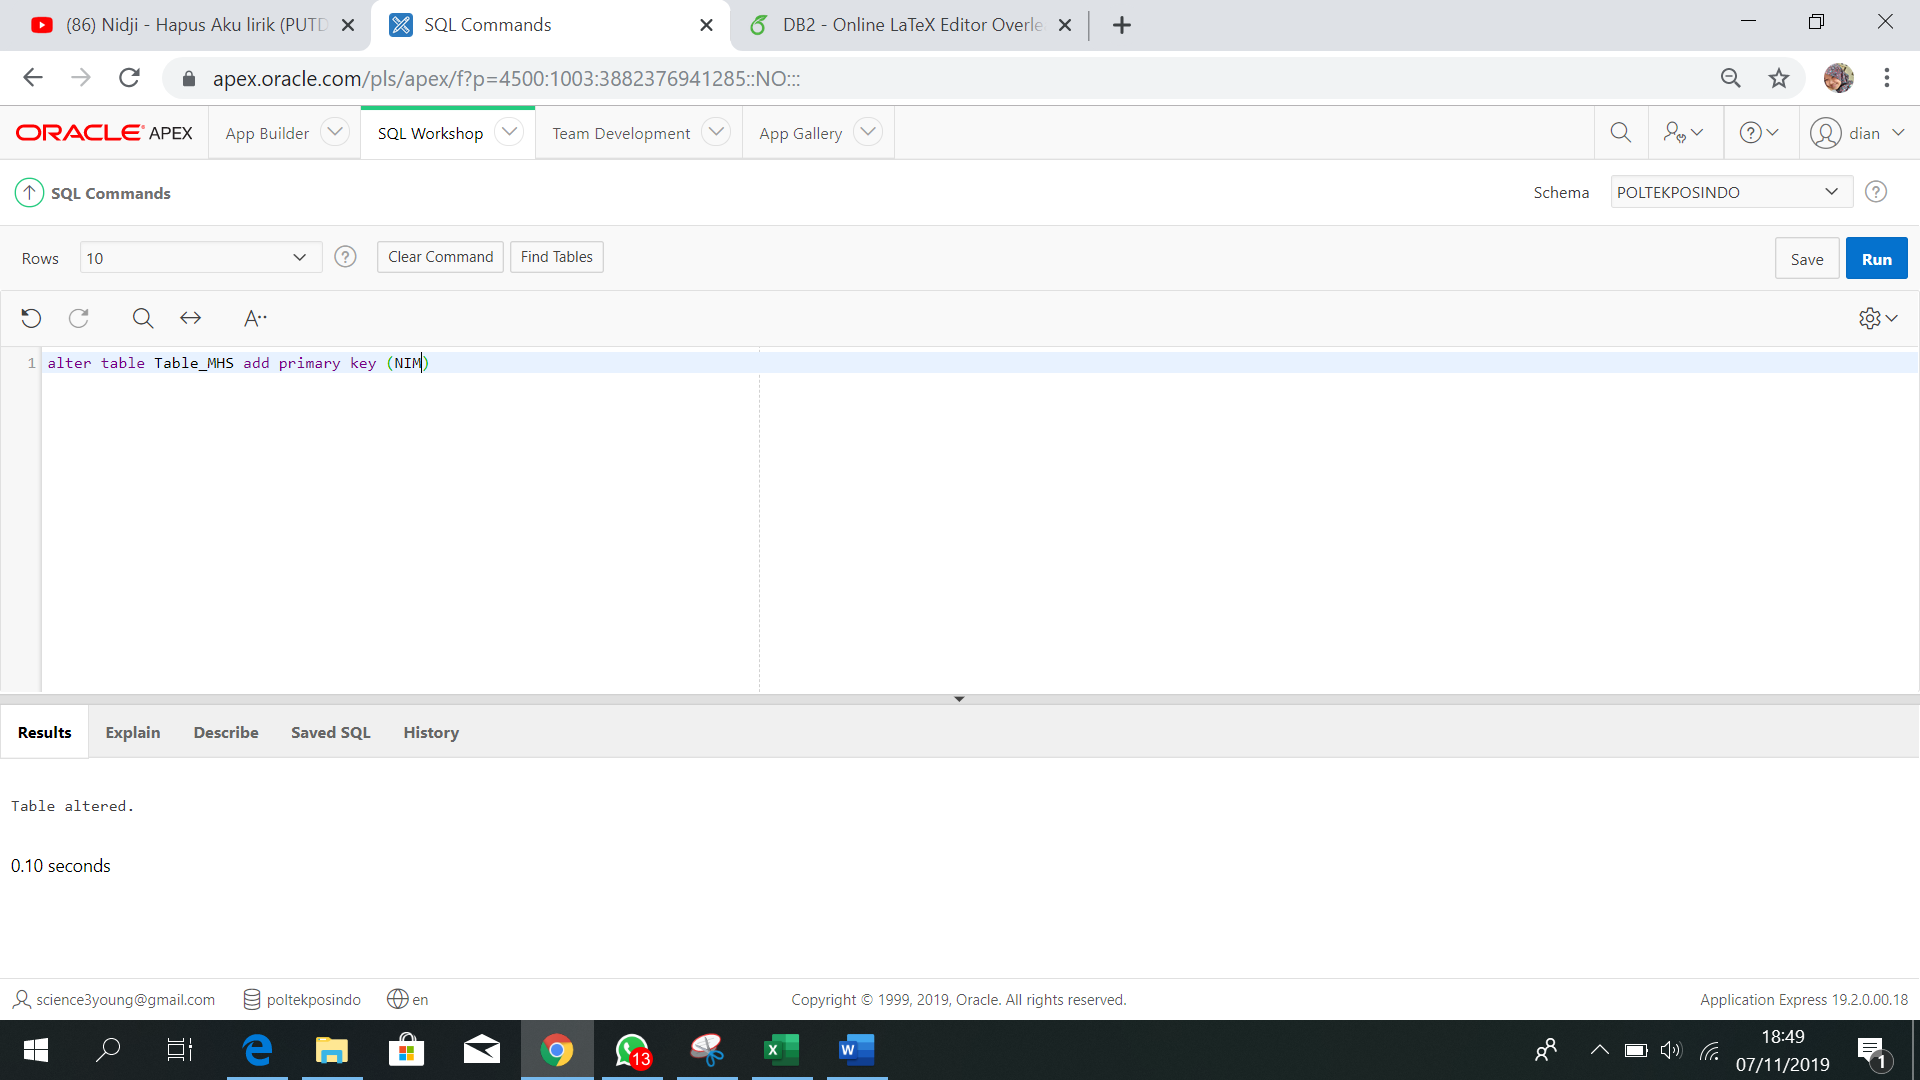
\includegraphics[width=15cm\textwidth]{figure/addpk.png}

\item 13.  Langkah selanjutnya adalah cara merelasikan dua tabel, yaitu kita mengetikan query\\

\item 14. Langkah selanjutnya kita ke app builder lalu klik create lalu klik new application 

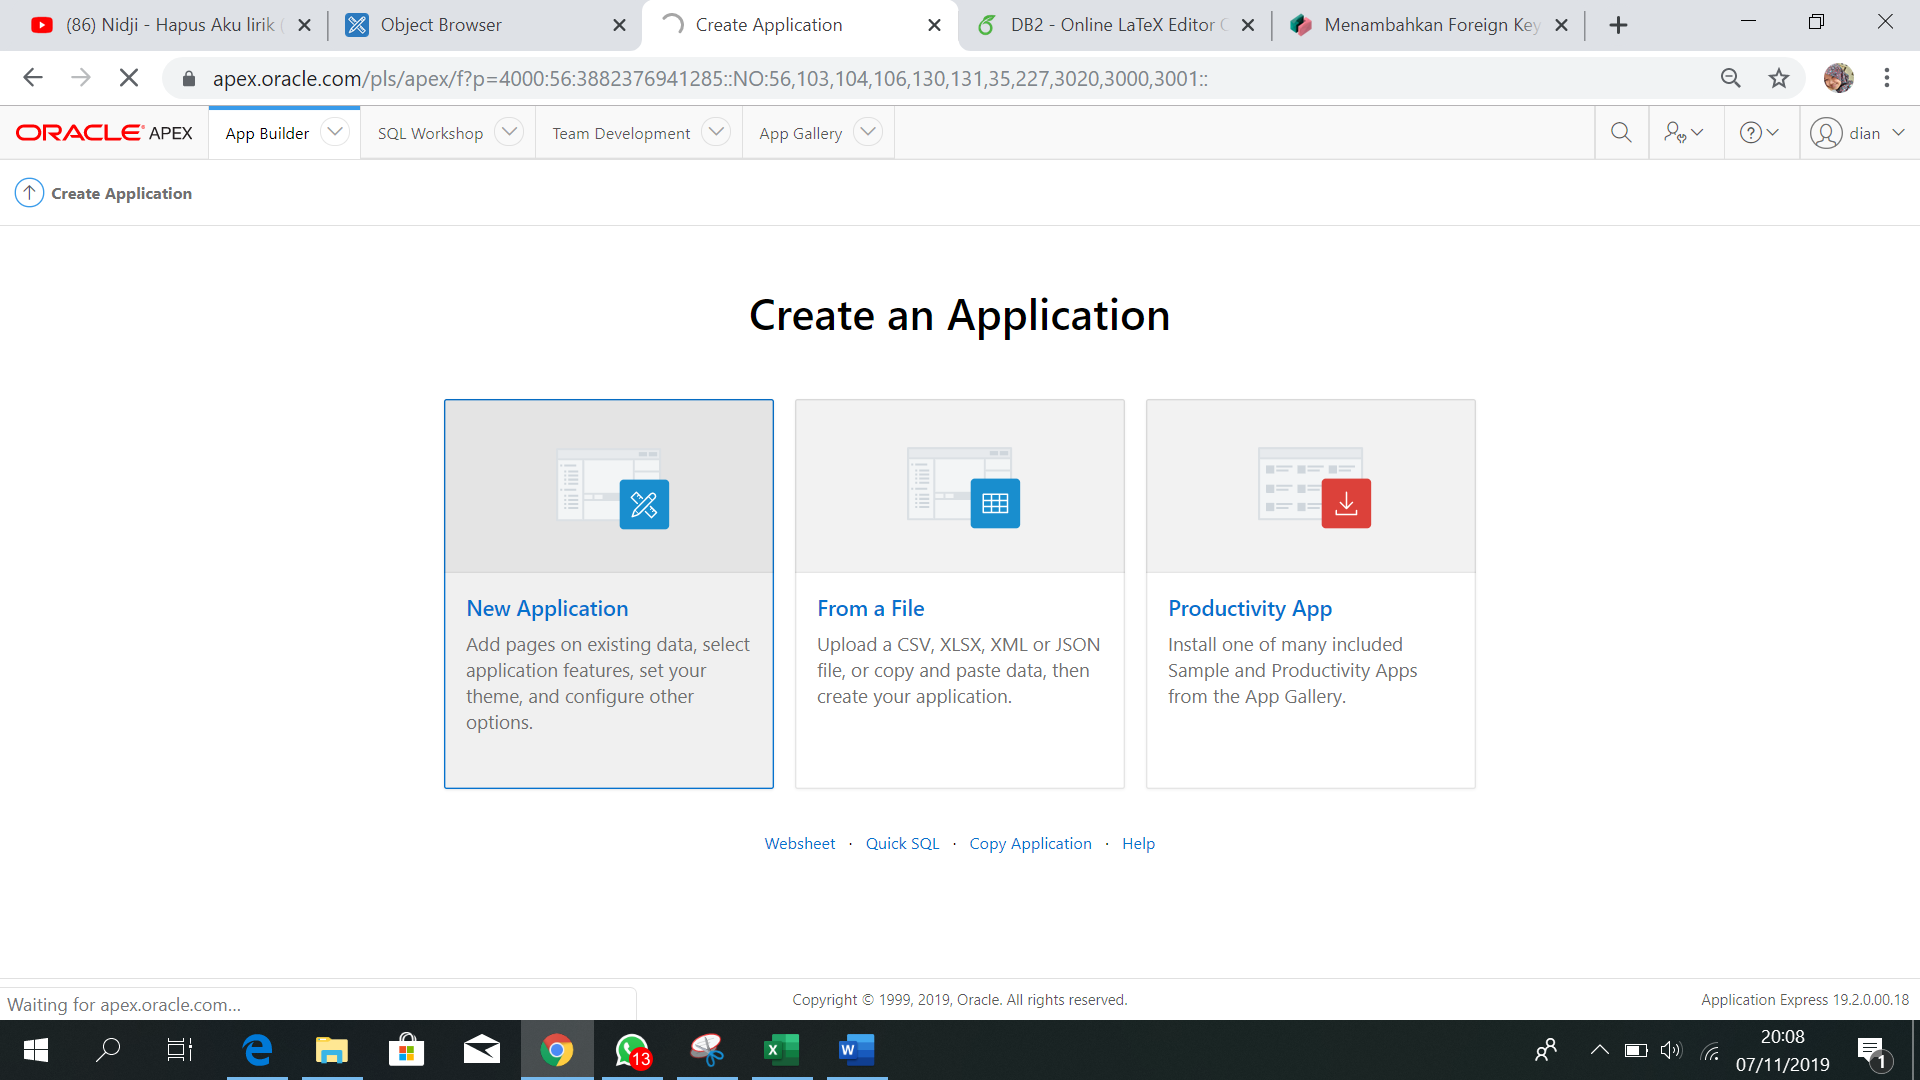
\includegraphics[width=15cm\textwidth]{figure/createapp.png}

\item 15. kemudian memberi nama aplikasi dan menambah halaman\\

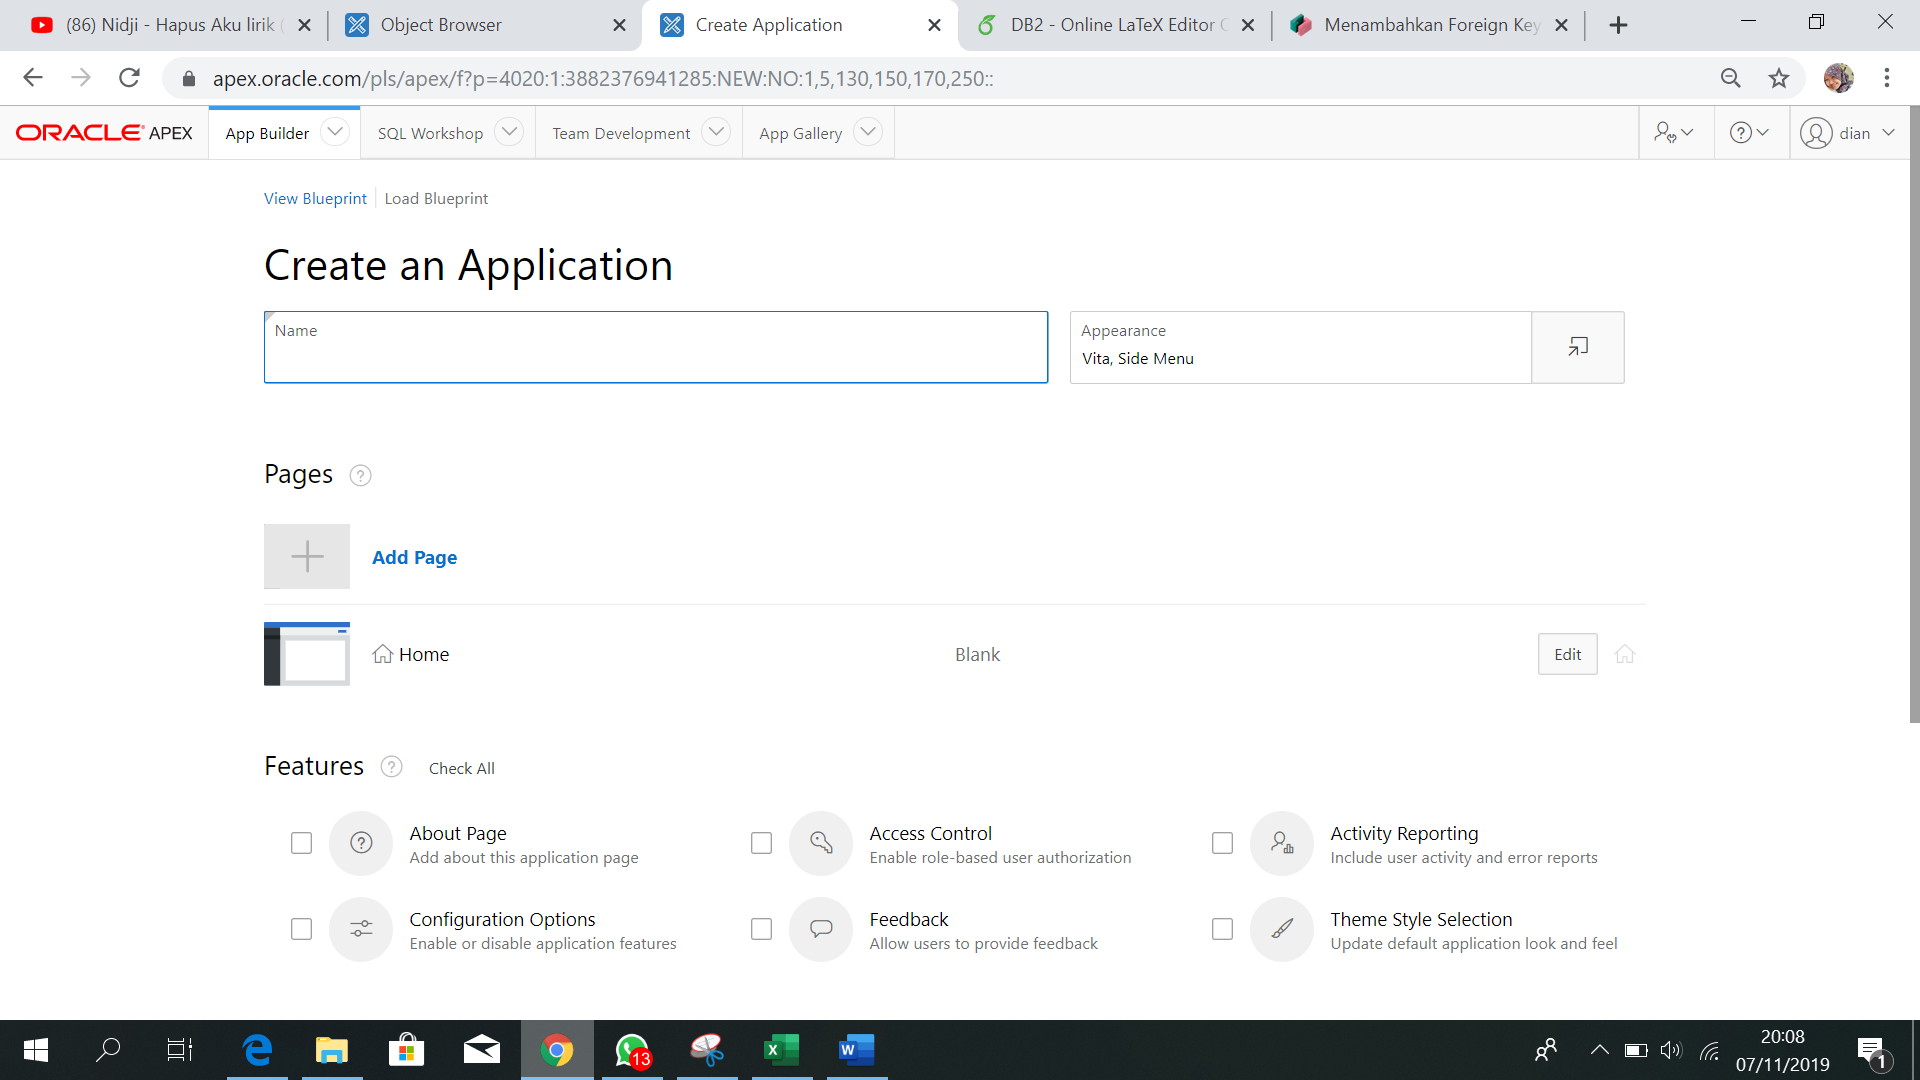
\includegraphics[width=15cm\textwidth]{figure/addpg.png}

\item 16. selanjutnya menambahkan tabel\\

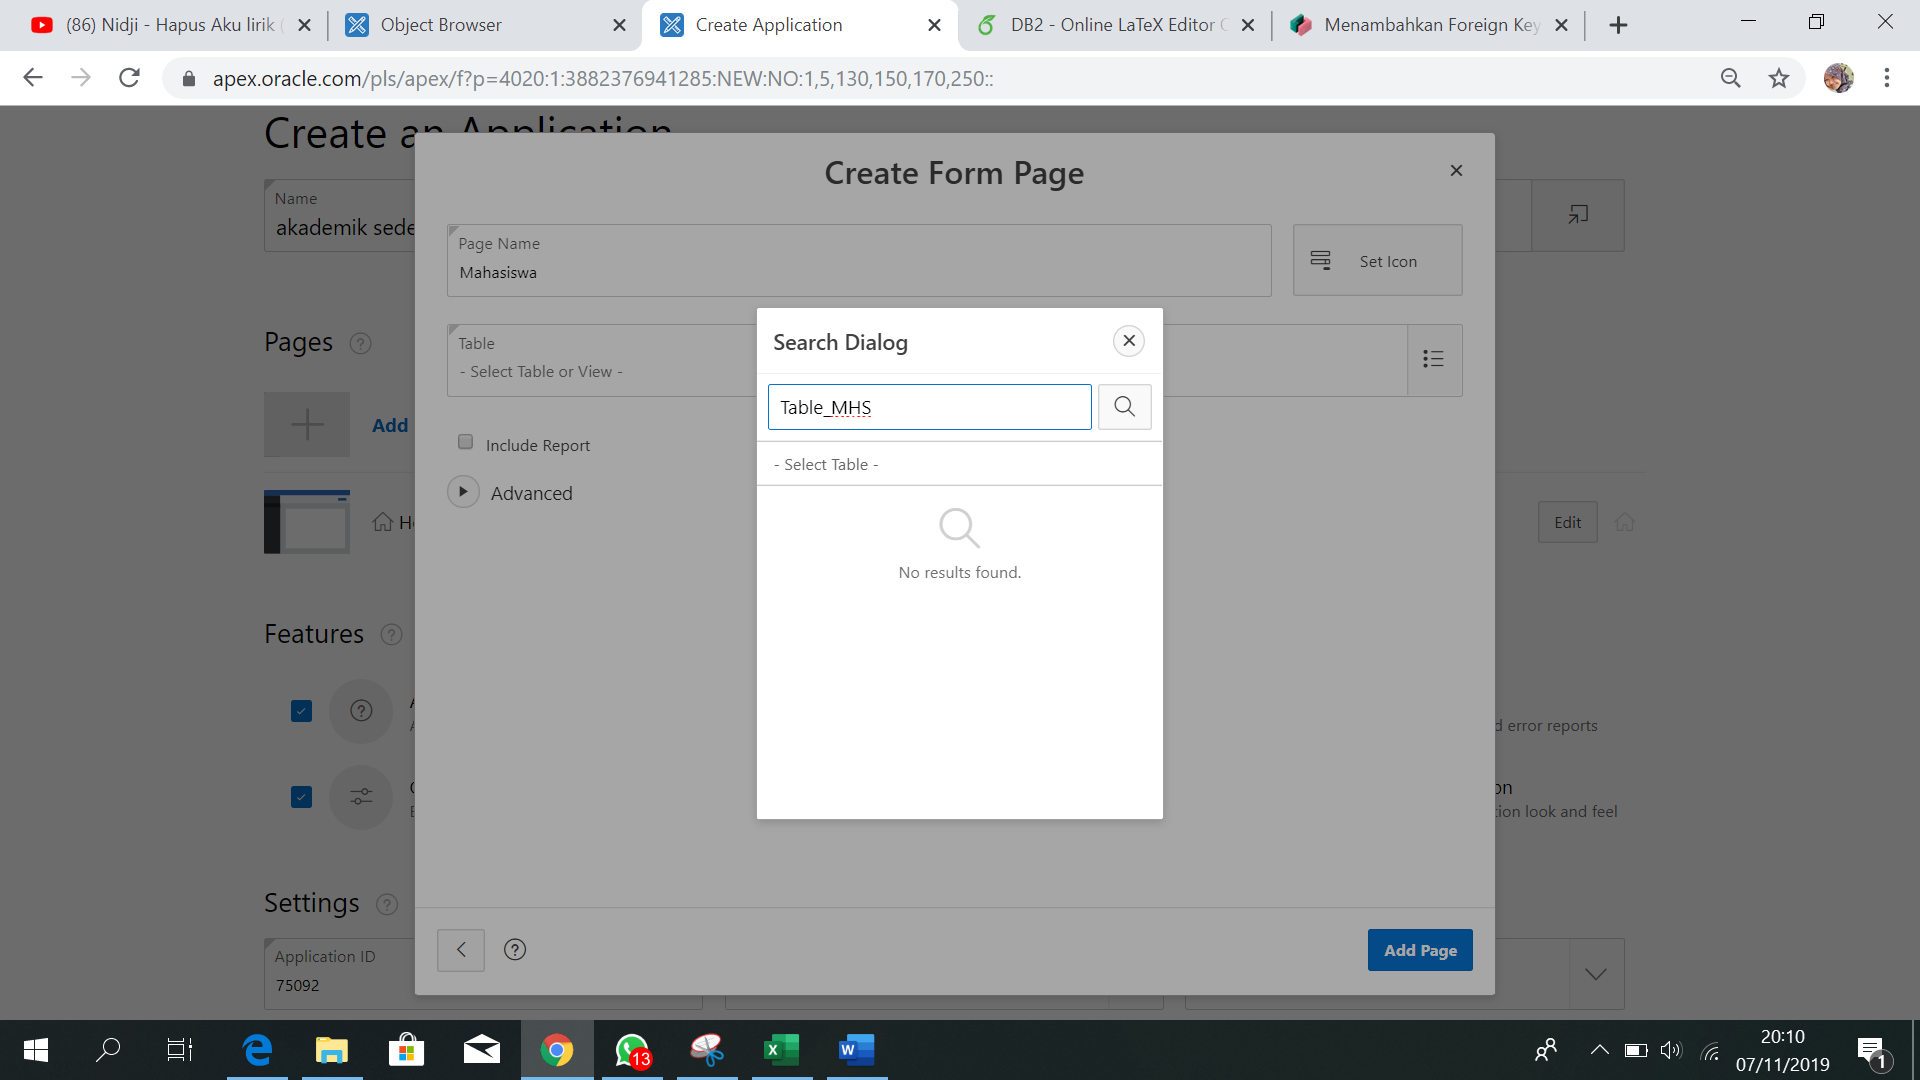
\includegraphics[width=15cm\textwidth]{figure/addtabel.png}

\item 17. create application final\\
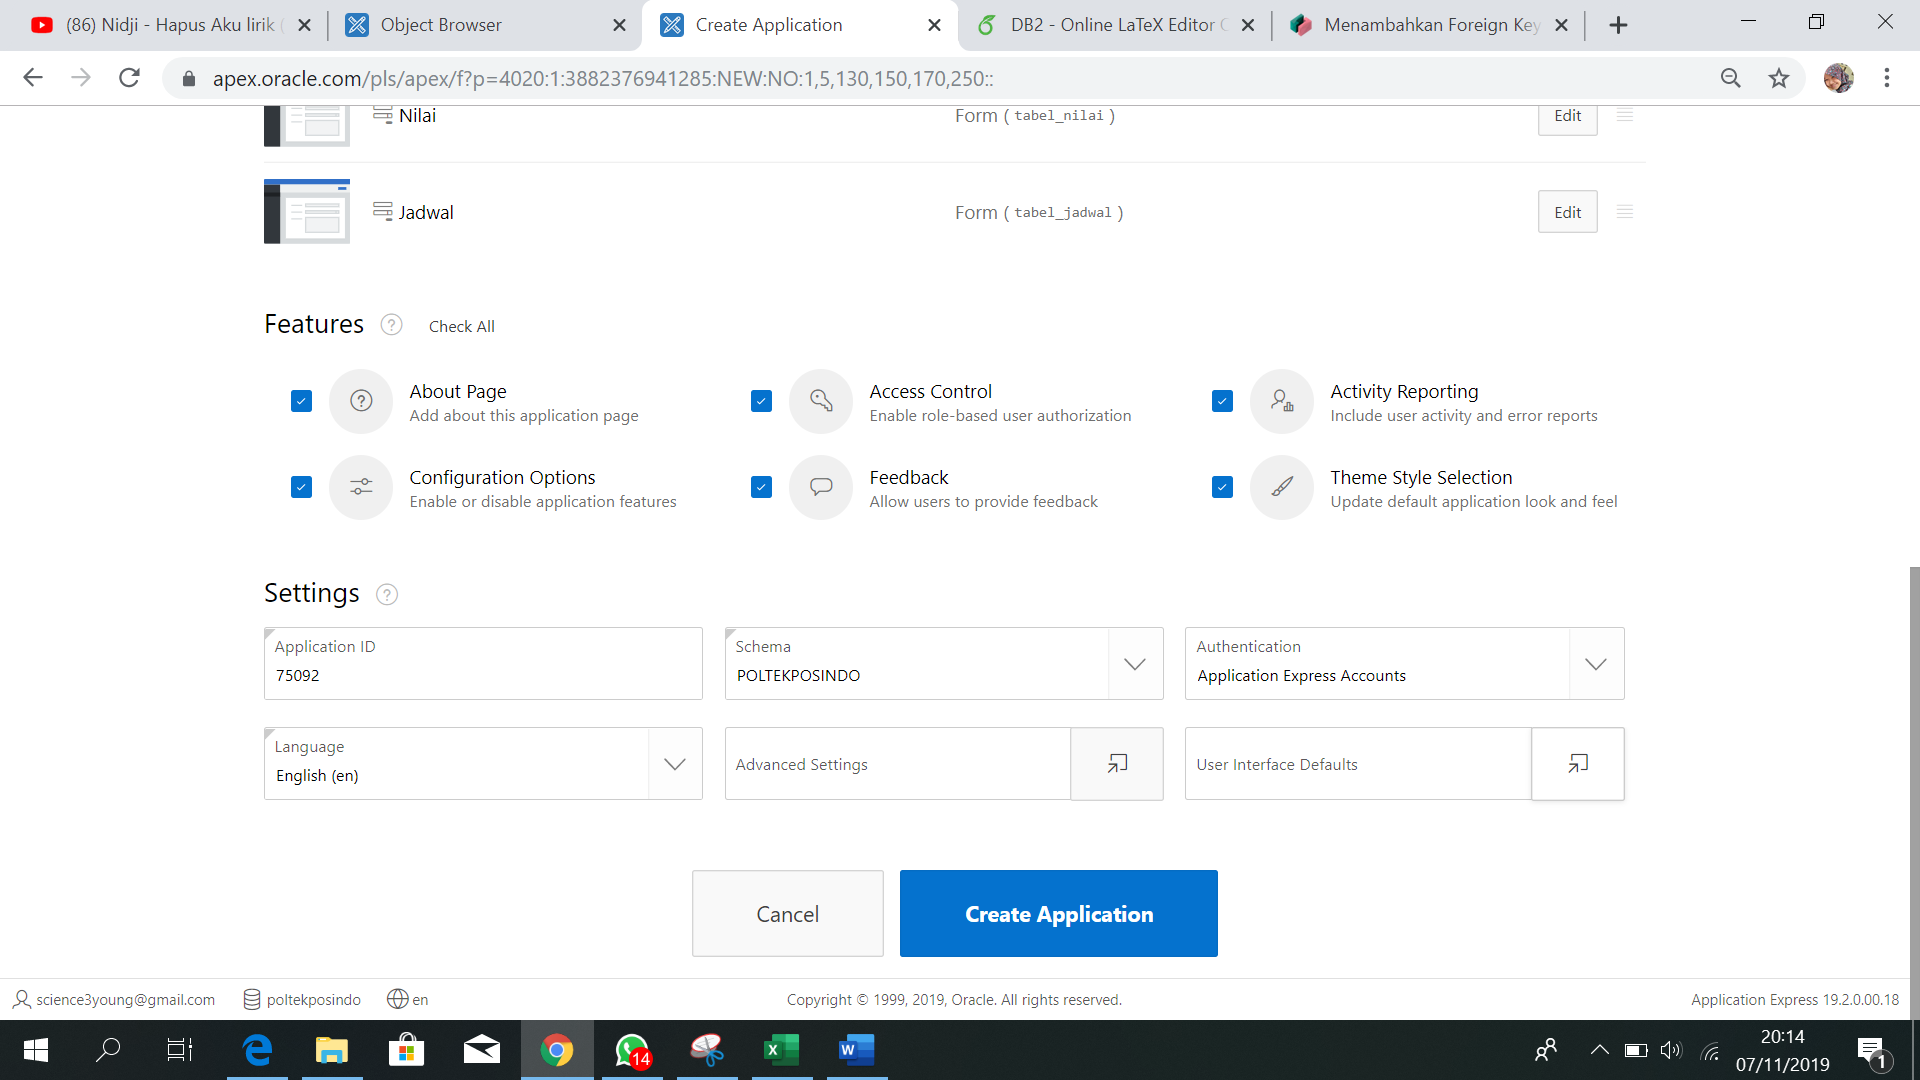
\includegraphics[width=15cm\textwidth]{figure/createappfinal.png}\\

\item 18. run application maka tampilannya seperti gambar dibawah ini\\
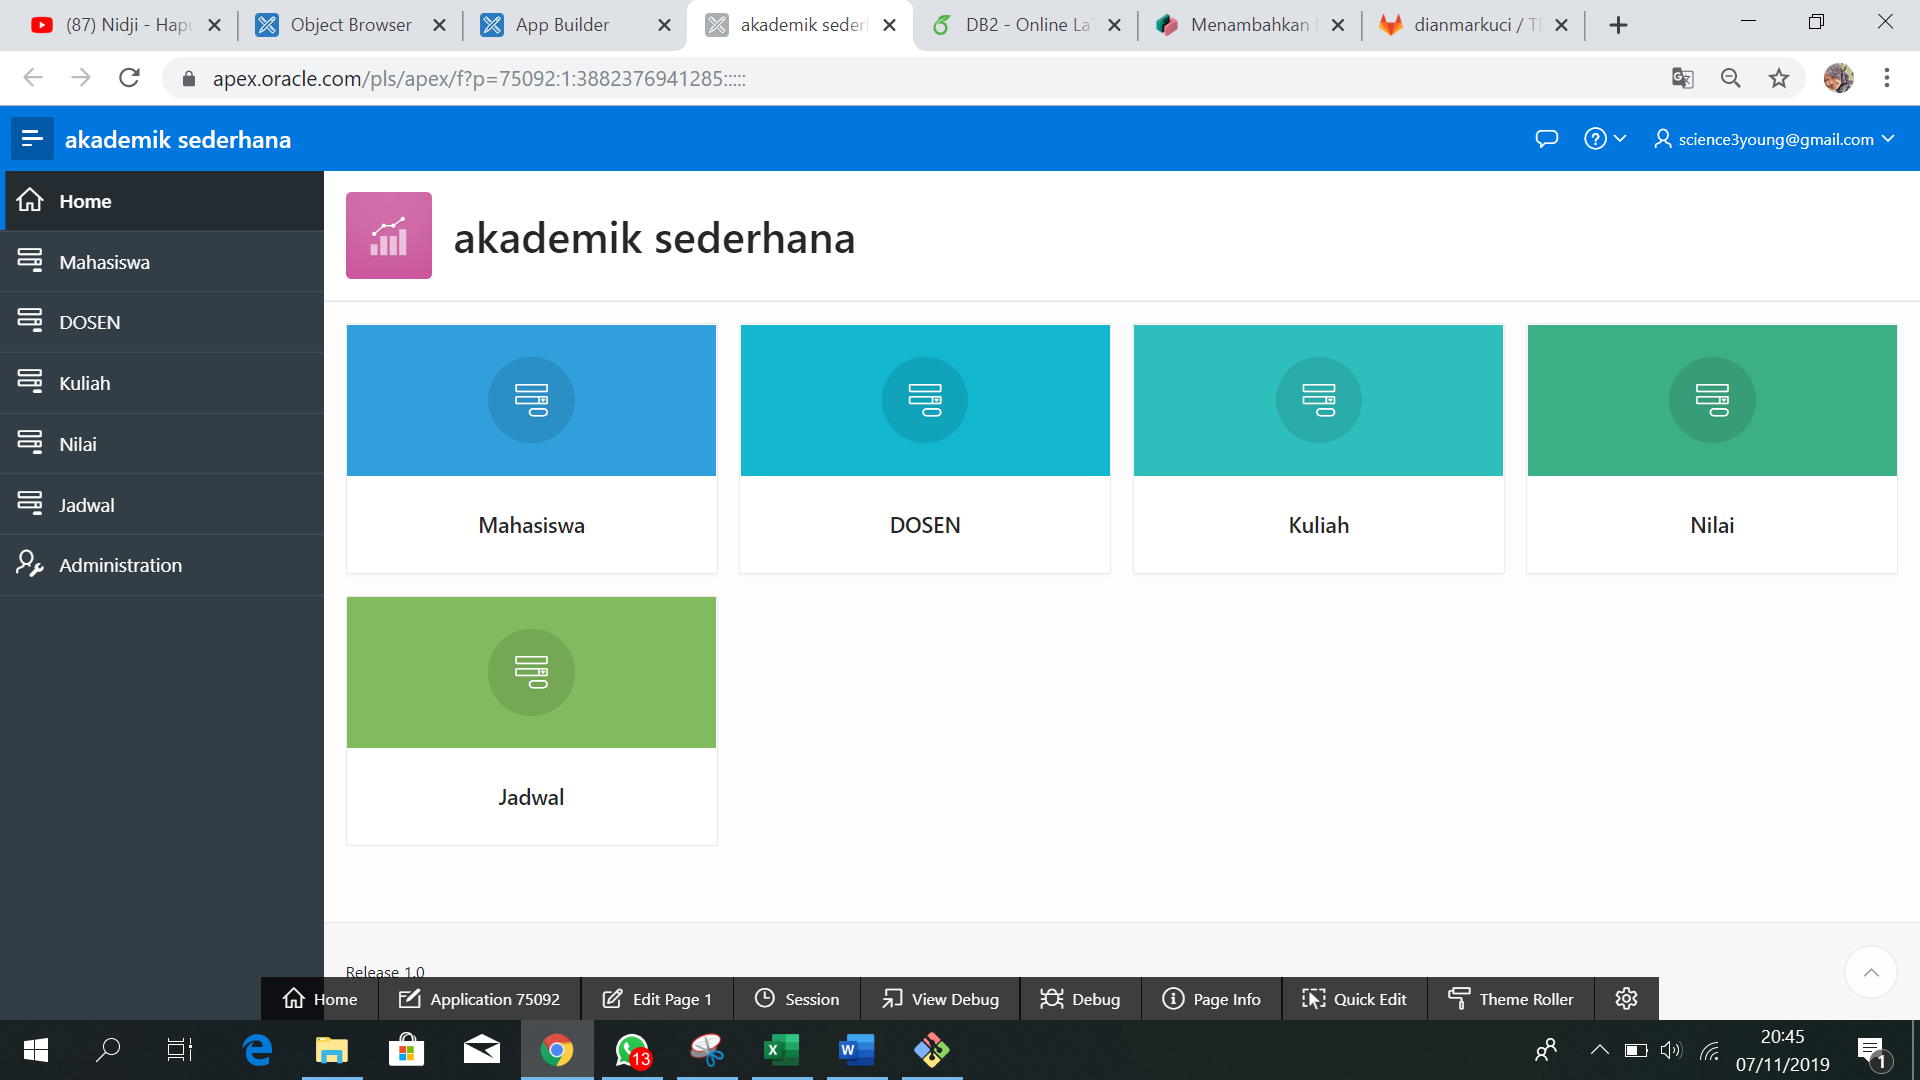
\includegraphics[width=15cm\textwidth]{figure/run.png}\\

SELESAI \\









link : https://apex.oracle.com/pls/apex/f?p=4550:1:711485402158908:::::\\
workspace: poltekposindo\\
username : science3young@gmail.com\\
password : dialine31\\
\end{document}


